\documentclass[a4paper]{report}

\usepackage{../mathstemplate}

\date{III семестр, осень 2023 г.}
\title{Дифференциальная геометрия. Неофициальный конспект}
\author{Лектор: Лебедева Нина Дмитриевна \\ Конспектировал Леонид Данилевич}

\begin{document}
    \shorthandoff{"}
    \maketitle
    \tableofcontents
    \newpage
    \setcounter{lection}{0}

    %Алгебраическая топология, кривые в $\R^2$ и в $\R^3$, двумерные поверхности в трёхмерном пространстве, риманова геометрия.


    \chapter{Алгебраическая топология}
    \newlection{4 сентября 2023 г.}


    \section{Применения фундаментальной группы}
    \theorem[Об инвариантности размерности края]{
        $\R^n$ не гомеоморфно никакому открытому подмножеству $U \subset \R^2$.
        \provehere{
            Рассмотрим произвольную точку $x \in U$.

            Если её удалить, то фундаментальная группа $U \sm \{x\}$ будет нетривиальной, а $\R^n \sm \{pt\}$ --- стягиваемо.
        }
    }
    \theorem[Об инвариантности края]{
        $\R_{\ge 0} \times \R$ не гомеоморфно никакому открытому $U \subset \R^2$.
        \provehere{
            У $\R_{\ge 0} \times \R$ можно выкинуть граничную точку, пространство останется стягиваемым.
        }
    }
    \definition[Ретракция топологического пространства $X \supset A$]{
        $f: X \map A$, такое, что $f\Big|_A = \id$.
    }
    \theorem[Борсук]{
        Не существует ретракции двумерного диска $D^2$ на свою границу $S^1 = \partial D^2$.
        \provehere{
            От противного. Рассмотрим композицию $S^1 \overset{\text{in}}\hookrightarrow D^2 \overset{f}{\map} S^1$.
            Композиция $\text{in} \circ f = \id_{S^1}$.

            Эта композиция индуцирует гомоморфизм фундаментальных групп, но у диска фундаментальная группа тривиальна.
        }
    }
    \note{
        Все предыдущие теоремы можно обобщить на случай больших размерностей, но в доказательстве будет уже не фундаментальная группа.
    }
    \theorem[Брауэр]{
        Любое непрерывное отображение $f: D^2 \map D^2$ имеет неподвижную точку.
        \provehere{
            От противного: $\exists f: D^2 \map D^2$ без неподвижных точек.

            Тогда можно построить ретракцию из диска на окружность: $x \in D^2$ отобразим в пересечение луча $f(x) \rightarrow x$ с границей $\partial D^2$.
            Назовём построенную функцию $g$.

            $g\Big|_{S^1} = \id$ по определению. Для проверки непрерывности запишем $g$ формулой:
            \[g(x) = f(x) + t_{x}(x - f(x))\]
            где $t_x$ выбирается так, что $|f(x) + t_x (x - f(x))| = 1$. Таким образом, $t_x$ --- положительный (больший) корень некоего квадратного уравнения с непрерывно меняющимися коэффициентами.
        }
    }
    \theorem[Основная теорема алгебры]{
        $\forall f \in \C[x]$, $\deg f \ge 1: \exists z_0 \in \C: f(z_0) = 0$.
        \provehere[Доказательство (дама с собачкой)]{
            Запишем $f(z) = z^n + a_1 z^{n -1} + \dots + a_n$.

            Обозначим $g(z) = a_1 z^{n-1} + \dots + a_n$.
            Выберем достаточно большое $R \in \R_+$, такое, что $|z| \ge R \then |z^n| > |g(z)|$.

            Если $z$ пробегает все значения одного модуля $z = R \cdot e^{i t}$ по $t \in [0, 2\pi]$, то $f(z) = z^n + g(z)$ пробегает некую нетривиальную петлю в $l \subset \C \sm \{0\}$ ($n$ раз оборачивающуюся вокруг нуля --- можно линейно прогомотопировать в петлю $R e^{i t}$).

            Рассмотрим гомотопию петли $\defset{R \cdot e^{it}}{t \in [0, 2\pi]} \subset \C$ в точку.
            Композиция $f$ с этой гомотопией создаст гомотопию петли $l$ в точку.
            Но в $\C \sm \{0\}$ $l$ не стягиваема, значит, применение $f$ заденет где-то $0$.
        }
    }
    \theorem[Улам-Борсук]{
        У любого $f: S^2 \map \R^2$ найдётся $x \in S^2: f(x) = f(-x)$.

        Предположим противное. Рассмотрим функцию $g(x) \coloneqq f(x) - f(-x)$. Это нечётная функция ($g(x) = -g(-x)$), мы предполагаем, что она не обнуляется.

        Сузим $g$ на экватор сферы. $g\Big|_{S^1}$ --- нечётная петля.
        \indentlemma{
            Нечётная петля имеет нечётный индекс (\textit{индекс} --- количество раз, которое петля обмоталась вокруг 0 с учётом ориентации).
        }{
            Рассмотрим $\alpha(x) = \frac{g(x)}{|g(x)|}$ --- отображение $S^1 \map S^1$, по-прежнему нечётное.

            Для определения индекса петли надо рассмотреть универсальное накрытие $\R \overset{p}\map S^1$.
            Обозначим за $\tilde(\alpha): [0, 2\pi] \map \R$ поднятие петли $\alpha$ ($\tilde{\alpha}(0) = \tilde{\alpha}(2\pi)$).

            Без потери общности можно считать, что $\tilde{\alpha}(0) = 0$.
            Так как $\alpha$ нечётная, то $\tilde{\alpha}(\pi) = \pi(2k + 1)$ для некоего $k \in \Z$.
            Дальше из нечётности $\alpha$ получаем $\tilde{\alpha}(2\pi) = 2\pi(2k + 1)$, что и значит нечётность индекса.
        }
        Аналогично предыдущей теореме, стянем экватор $S^1$ в точку, петля стянется в точку, значит, где-то заденет $0$.
    }


    \section{Теорема Жордана}
    \theorem[Детская версия теоремы Жордана]{
        Рассмотрим диск $D^2$, пусть $N$ и $S$ --- северный и южный полюса диска соответственно.

        Пусть $\gamma_0: [0, 1] \map \D^2$ --- путь от $N$ до $S$, причём пусть $\gamma_0(0, 1) \cap S^1 = \o$.

        Тогда существуют $p, q \in D^2$, <<достаточно близкие к границе>>, такие, что $p$ и $q$ лежат в разных компонентах связности $D^2 \sm \Image(\alpha)$.
        \provehere{
            Выберем $p_0$ на дуге $NS$ и $q_0$ на дуге $SN$.
            Выберем внутри диска достаточно близко к $p_0$ и $q_0$, точки $p$ и $q$ соответственно (выберем так, чтобы $p_0$)
        }
    }
    \theorem[Теорема Жордана]{
        Рассмотрим инъективное $S^1 \overset{\alpha}\hookrightarrow \R^2$. Тогда число компонент связности $\#(\R^2 \sm \Image(\alpha)) = 2$.
    }
    \note[Уточнение, теорема Шёнфлиса]{
        Эти компоненты связности гомеоморфны компонентам связности $\R^2 \sm S^1$.
    }


    \section{Ретракция. Гомотопическая эквивалентность}
    Как уже было сказано,
    \definition[Ретракция топологического пространства $X \supset A$]{
        $f: X \map A$, такое, что $f\Big|_A = \id$.
    }

    \theorem{
        Пусть существует $r: X \map A$ --- ретракция. Тогда для отображения $\text{in}: A \map X$ индуцированный гомоморфизм фундаментальных групп $\text{in}_*$ инъективен.
        \provehere{
            Композиция $A \overset{\text{in}}\map X \overset{r}\map A$ тождественна, значит, индуцированный гомоморфизм фундаментальных групп тождественнен, значит, никакие точки при $\text{in}_*$ не склеились.
        }
    }
    \definition[Деформационная ретракция $X \supset A$]{
        Гомотопия $H: X \times [0, 1] \map X$, такое, что $\forall a \in A, t \in [0, 1]: H(a, t) = a$, причём $H(\_, 1) = A$.
    }
    \note{
        Некоторые определения не такие сильные --- требуют $H(a, t) \in A$ или даже только $H(a, 1) = a$.
    }
    \newlection{11 сентября 2023 г.}
    \precaution[Проблемы с доказательством теоремы Жордана]{
        Длина кривой может быть бесконечной.
        Кривая может бесконечно закручиваться, как спираль, внутрь себя. (?)
        Заменить кривую на ломаную может не получиться, так как будут возникать самопересечения.
    }
    \lemma{
        Пусть $p, q$ --- концы пути $\gamma$, причём петля $\alpha$ не пересекается с носителем пути $\gamma$.
        Тогда $\text{ind}_p(\alpha) = \text{ind}_q(\alpha)$.
        \provehere{
            Рассмотрим гомотопию $H(x, t) = \alpha(x) - \gamma(t)$. Это непрерывная деформация $\alpha$, которая не задевает 0, значит, индексы $p$ и $q$ равны.
        }
    }
    \theorem[Шёнфлис, для ломаных]{
        Пусть $\alpha$ --- замкнутая несамопересекающаяся ломаная с вершинами $A_1, \dots, A_n$.

        Тогда плоскость бьётся на две компоненты связности, одна гомеоморфна $B_1(0)$, другая --- $\R^2\sm D_1(0)$.
        \provebullets{
            \item Докажем, что компонент связности $\R^2 \sm \Image(\alpha)$ не больше 2.
            Зафиксируем точку $p$ на границе, у неё есть окрестность, гомеоморфная $B_2$ без диаметра.

            Любую другую точку $q$ можно соединить с этой окрестностью путём, не пересекающим $\Image(\alpha)$ --- подойдём достаточно близко к кривой, дальше будем идти вдоль неё.

            Так как компонент связности $B_2$ без диаметра две, то и компонент связности $\R^2 \sm \Image(\alpha)$ не больше 2.
            \item Пусть $l$ --- прямая, не параллельная $A_i A_j$ для всех пар $i \ne j$.
            Пусть $N$ --- нормаль к $l$.
            Определим функцию высоты $h(p) = \angles{N, p}$.
            У всех точек $A_1, \dots, A_n$ разная высота.

            Зафиксируем высоту $h$, рассмотрим точки пересечения $B_1, \dots, B_k$ ломаной $\alpha$ с линией уровня $h$.
            Каждой вершине $B_1, \dots, B_k$ сопоставим чётность --- $0$, если в окрестности этой вершины уровни ломаной всегда не больше (или не меньше), чем уровень данной точки.
            Иначе --- если уровень ломаной меняет знак в данной вершине --- присвоим чётность $1$.

            Каждой точке на линии уровня $h$ присвоим чётность, равную сумме (в $\Z/2\Z$) чётностей вершин левее.
            Точки с чётностями $0$ лежат снаружи ломаной, с чётностями $1$ --- внутри.

            По построению очевидно, что точки разных чётностей лежат в разных компонентах связности $\R^2\sm\Image(\alpha)$ (отображение $\R^2\sm\Image(\alpha) \map \{0, 1\}$, сопоставляющее точке уровень непрерывно, что проверяется ручками), а так как компонент связности не больше 2, то их ровно 2.
            \item Докажем, что множество <<нечётных точек>> гомеоморфно $B_2$.
            Для этого триангулируем их замыкание --- на самом деле, <<нечётные точки>>, объединённые с $\Image(\alpha)$.

            Проведя все линии уровня для $h \in \{h(A_1), \dots, h(A_n)\}$, мы получим разбиение на множество треугольников и трапеций --- трапеции несложно триангулировать.

            Склейка множества треугольников по рёбрам, как известно, даёт сферу с ручками, дырками и плёнками.

            Плёнки получиться не могут --- они неориентируемы, а $\R^2$ ориентируема.
            Но и ручки получиться не могут --- в предположении, что из плоскости получилось вырезать ручку, мы можем устроить (не деформационную) ретракцию из плоскости на окружность, что противоречит тому, что у окружности фундаментальная группа больше.
            Для этого представим ручку, как тор с дыркой --- $S^1 \times S^1$ с дыркой.
            Ретракция на окружность устроена отбрасыванием второй координаты.

            У каждой дырки есть компонента края.
            То, что дырок ровно одна понятно из того, что край --- как-раз-таки только та ломаная $\alpha$.
            Но ломаная связна, значит, компонента края одна.
        }
    }


    \section{Гомотопическая эквивалентность}
    Пусть $X, Y$ --- топологические пространства.
    \definition[Гомотопически обратные отображения]{
        Отображения $f: X \map Y, g: Y \map X$, такие, что $f \circ g \sim \id_Y$ и $g \circ f \sim \id_X$.
    }
    \definition[Гомотопически эквивалентные пространства]{
        Такие $X, Y$, что $\exists f: X \map Y, g: Y \map X$ --- гомотопически обратные отображения.

        Обозначается $X \sim Y$.
    }
    \theorem{
        Пусть $X$ --- деформационный ретракт $Y$ (достаточно самого слабого определения).
        Тогда $X \sim Y$.
        \provehere{
            Пусть $\tau: Y \map X$ --- ретракция, $\text{in}: X \map Y$ --- включение.

            Докажем, что $\tau$ и $\text{in}$ --- гомотопически обратные.
            \bullets{
                \item $\tau \circ \text{in} = \id_X$, поэтому и гомотопически эквивалентно $X$.
                \item $\text{in} \circ \tau \sim \id_Y$ по определению деформационной ретракции.
            }
        }
    }
    \examples[Гомотопически эквивалентные пространства]{
        \item $[0, 1] \sim [0, 1]\times[0, 1]$ --- отрезок является деформационным ретрактом квадрата.
        \item $(S^1 \sim \text{лист Мёбиуса})$.
        \item Точка гомотопически эквивалентна дереву.
        \item Две разные (одномерные) восьмёрки гомомотопически эквивалентны, потому что они --- ретракты третьей (двумерной) восьмёрки~(\ref{eights}).
        \pic[0.4]{eights}{Восьмёрки}
    }
    \theorem{
        Гомотопическая эквивалентность --- отношение эквивалентности.
        \provebullets{
            \item Рефлексивность: $X \sim X$, так как $\id_X$ и $\id_X$ --- гомотопически обратные.
            \item Симметричность заложена в определение.
            \item Транзитивность:
            пусть $X \underset{h}{\overset{f}\rightleftarrows} Y \underset{i}{\overset{g}\rightleftarrows} Z$, где $g \circ i, i \circ g, f \circ h$ и $h \circ f$ гомотопны постоянным отображениям соответвующего пространства.
            Таким образом, так как $i \circ g \sim \id_Y$, то \[h \circ (i \circ g) \circ f \sim h \circ f \sim \id_X\]
            Аналогично $g \circ f \circ h \circ i \sim \id_Z$.
        }
    }


    \section{Пары Борсука}
    \definition[$(X, A)$ --- пара Борсука]{
        $A \subset X$, причём $\forall Y: \forall f: X \map Y: \forall H: A \times I \map Y: H(\_, 0) = f\Big|_A(\_)$ эту гомотопию можно продолжить: $\exists \tilde{H}:X \times I \map Y$, такая что $\tilde{H}\Big|_{A \times I} = H$, причём $\tilde{H}(\_, 0) = f(\_)$.
    % https://q.uiver.app/#q=WzAsNSxbMCwwLCJBIl0sWzEsMSwiWCBcXHRpbWVzIEkiXSxbMSwwLCJYIl0sWzAsMSwiQSBcXHRpbWVzIEkiXSxbMiwyLCJZIl0sWzMsNCwiSCIsMCx7ImN1cnZlIjoyfV0sWzIsNCwiZiIsMCx7ImN1cnZlIjotMn1dLFswLDIsIiIsMix7InN0eWxlIjp7InRhaWwiOnsibmFtZSI6Imhvb2siLCJzaWRlIjoidG9wIn19fV0sWzEsNCwiXFx0aWxkZXtIfSIsMCx7InN0eWxlIjp7ImJvZHkiOnsibmFtZSI6ImRhc2hlZCJ9fX1dLFsyLDEsIiIsMCx7InN0eWxlIjp7InRhaWwiOnsibmFtZSI6Imhvb2siLCJzaWRlIjoiYm90dG9tIn19fV0sWzAsMywiIiwwLHsic3R5bGUiOnsidGFpbCI6eyJuYW1lIjoiaG9vayIsInNpZGUiOiJ0b3AifX19XSxbMywxLCIiLDEseyJzdHlsZSI6eyJ0YWlsIjp7Im5hbWUiOiJob29rIiwic2lkZSI6InRvcCJ9fX1dXQ==
        \[\begin{tikzcd}[ampersand replacement=\&]
              A \& X \\
              {A \times I} \& {X \times I} \\
              \&\& Y
              \arrow["H", curve={height=12pt}, from=2-1, to=3-3]
              \arrow["f", curve={height=-12pt}, from=1-2, to=3-3]
              \arrow[hook, from=1-1, to=1-2]
              \arrow["{\tilde{H}}", dashed, from=2-2, to=3-3]
              \arrow[hook', from=1-2, to=2-2]
              \arrow[hook, from=1-1, to=2-1]
              \arrow[hook, from=2-1, to=2-2]
        \end{tikzcd}\]
    }
    \newlection{18 сентября 2023 г.}
    В некотором смысле, практически все пары пространства-подпространства, которые естественно придумать, являются парой Борсука.

    \fact{
        Пусть $X \supset A$, причём $B$ локально компактно.
        Тогда $(X/A) \times B \equiv (X \times B)/_{(a_1, b) \sim (a_2, b)}$.
        \provehere{
            Равенство множеств проверить несложно, но чтобы поверить гомеоморфизм топологических пространств, надо воспользоваться локальной компактностью.

            Этот факт из общей топологии мы доказывать не будем.
        }
    }
    \note{
        $A$ --- стягиваемо $\iff \forall a \in A$: $a$ --- деформационный ретракт $A$ в самом слабом смысле.
    }
    \theorem{
        Пусть $(X, A)$ --- пара Борсука. Если $A$ стягиваемо, то $X \sim X/A$.
        \provehere{ Пусть $\mathcal{F}^*: A \times I \map A$ --- гомотопия, стягивающая $A$ в точку $a \in A$ (таким образом $\mathcal{F}^*\Big|_{A \times \{0\}} = \id$ и $\mathcal{F}^*\Big|_{A \times \{1\}} = a$)

            Положим в качестве $\mathcal{F}$ гомотопию, продолжающую $\mathcal{F}^*$ так, что $\mathcal{F}\Big|_{X \times \{0\}} = \id$ (такая найдётся по определению пары Борсука).

            Так как $\forall t \in I: (p \circ \mathcal{F})(A, t) \subset A$, то $p \circ \mathcal{F}$ пропускается через фактор:
            существует непрерывное $\tilde{\mathcal{F}}$, делающее диаграмму коммутативной.
        % https://q.uiver.app/#q=WzAsNSxbMCwyLCIoWCBcXHRpbWVzIEkpL197KGFfMSwgdCkgXFxzaW0gKGFfMiwgdCl9Il0sWzIsMiwiWC9BIl0sWzAsMCwiWCBcXHRpbWVzIEkiXSxbMiwwLCJYIl0sWzEsMSwiKFgvQSkgXFx0aW1lcyBJIl0sWzAsMSwiXFx0aWxkZXtcXG1hdGhjYWx7Rn19IiwyXSxbMiwwLCJcXHRpbGRle3B9IiwyXSxbMywxLCJwIl0sWzIsMywiXFxtYXRoY2Fse0Z9Il0sWzIsNCwiKHAsIFxcaWQpIiwxXSxbNCwxLCJcXHRpbGRle1xcbWF0aGNhbHtGfX0iXSxbMCw0LCJcXGNvbmciLDEseyJzdHlsZSI6eyJ0YWlsIjp7Im5hbWUiOiJhcnJvd2hlYWQifX19XV0=
            \[\begin{tikzcd}[ampersand replacement=\&]
            {X \times I}
                  \&\& X \\
                  \& {(X/A) \times I} \\
                  {(X \times I)/_{(a_1, t) \sim (a_2, t)}} \&\& {X/A}
                  \arrow["{\tilde{\mathcal{F}}}"', from=3-1, to=3-3]
                  \arrow["{\tilde{p}}"', from=1-1, to=3-1]
                  \arrow["p", from=1-3, to=3-3]
                  \arrow["{\mathcal{F}}", from=1-1, to=1-3]
                  \arrow["{(p, \id)}"{description}, from=1-1, to=2-2]
                  \arrow["{\tilde{\mathcal{F}}}", from=2-2, to=3-3]
                  \arrow["\cong"{description}, tail reversed, from=3-1, to=2-2]
            \end{tikzcd}\]
            Дальше надо сказать ещё немало (?) слов, что-то из них написано ниже.
            \indent{
                Так как $(X \times I)/_{(a_1, t) \sim (a_2, t)} \cong (X/A) \times I$, то можно считать, что $\tilde{F}$ бьёт из $(X/A) \times I$ в $X/A$.
                Пусть $p: X \map X/A$, $q : X/A \map X$, причём $p \circ q: X/A \map X/A$ и $q \circ p: X \map X$ гомотопно постоянному.

                Пусть $\mathcal{F}^{**}: A \times I \map A$, $\mathcal{F}^*: \text{in}_{A \hookrightarrow X} \circ \mathcal{F}^{**}, A \times I \map X$.

                Пусть $\mathcal{F}$ --- гомотопное продолжение $\mathcal{F}^*, \mathcal{F}\Big|_{X \times \{0\}} = \id$.

                $\mathcal{F}: X \times I \map X \overset{p}\map X/A$.

% https://q.uiver.app/#q=WzAsMyxbMCwwLCJYIl0sWzEsMCwiWCJdLFswLDEsIlgvQSJdLFswLDIsInAiLDJdLFsyLDEsInEiLDJdLFswLDEsIlxcbWF0aGNhbHtGfV8xIiwyXV0=
                \[\begin{tikzcd}[ampersand replacement=\&]
                      X \& X \\
                      {X/A}
                      \arrow["p"', from=1-1, to=2-1]
                      \arrow["q"', from=2-1, to=1-2]
                      \arrow["{\mathcal{F}_1}"', from=1-1, to=1-2]
                \end{tikzcd}\]

                $p \circ F: X \times I \map X/A$, это можно непрерывно пропустить через фактор $\mathcal{F}^\sim: (X \times I)/\sim \map X/A$.}
        }
    }
    \ok
    % Солнышко гомотопически эквиваелнтно перекрёстку. Восьмёрки гомотопчисеки эквивалентны друг другу.


    \section{Клеточная пара --- пара Борсука}
    Пусть $X$ --- клеточное пространство, $A \subset X$ --- замкнутое подпространство, состоящее из целого числа клеток.
    \fact{
        Пусть $A$ замкнуто в $X$ (необязательное условие, без которого сложнее).

        Рассмотрим пространство $X \times I$.
        $A \subset X$ --- пара Борсука, если $(X \times \{0\}) \cup (A \times I)$ --- ретракт $X \times I$.
        \provehere{
            Обозначим данную ретракцию за $\rho: X \times I \map (X \times \{0\} \cup A \times I)$.
            Чтобы показать, что $(X, A)$ --- пара Борсука, рассмотрим произвольное $f: X \map Y$, рассмотрим гомотопию $H: A \times I \map Y$, такую, что $H\Big|_{A \times \{0\}} = f\Big|_A$.

            Необходимо показать существование продолжения гомотопии $\tilde{H}: X \times I \map Y$.
            Подойдёт \[\tilde{H}: (x, t) \mapsto \all{f(\tilde{x}),&\rho(x) = (\tilde{x}, 0) \in X \times \{0\}\\ H(a, t),&\rho(x) = (a, t) \in A \times I}\]
            Непрерывность $\tilde{H}$ следует из замкнутости $A$ в $X$.
        }
    }
    \note{
        $(D^n, \partial D^n) = (D^n, S^{n - 1})$ --- пара Борсука.
        \provehere{
            Цилиндр $D^n \times I$ легко можно стянуть на <<стакан>> $(D^n \times \{0\}) \cup (S^{n - 1} \times I)$.

            Пусть $y$ --- центр шара $D^n$.
            Ретракция может быть устроена следующим образом:
            \begin{align*}
                H: D^n \times I &\map (D^n \times \{0\}) \times (S^{n - 1} \times I)\\(x, t) &\mapsto \all{\left(y + (x - y) \cdot \frac{2 - t}{d(x, y)},\frac{2 - t}{d(x,y)}\right),&\frac{2 - t}{d(x, y)} \le 2\\\left(y + (x - y) \cdot \frac{2}{2 - t},0\right),&\frac{2 - t}{d(x, y)} \ge 2}
            \end{align*}
            Иначе говоря, берётся произведение диска $D^n \subset \R^n$ с отрезком $[0, 2]$, в качестве стакана выбирается $(D^n \times \{0\}) \cup (\partial D^n \times [0, 1])$, после чего все точки $x \in D^n \times [0, 1]$ переходят в пересечение луча $(0, 2) \rightarrow x$ и стакана.
        }
    }
    \note{
        Если $(X, A)$ и $(A, B)$ --- пары Борсука, то $(X, B)$ --- пара Борсука.
        \provehere{
            Прямо из определения.
            Пусть $f: X \map Y$, $H: B \times I \map Y$ --- отображение и гомотопия, которые надо продолжить $f\Big|_{B} = H\Big|_{B \times \{0\}}$.

            Так как $(A, B)$ --- пара Борсука, то $\exists H_1: A \times I \map Y$, такая, что $H_1\Big|_{B \times I} = H, H_1\Big|_{B \times \{0\}} = f\Big|_{B}$.

            Так как $(X, A)$ --- пара Борсука, то $\exists H_2: X \times I \map Y$, такая, что $H_2\Big|_{A \times I} = H_1, H_2\Big|_{A \times \{0\}} = f\Big|_{A}$.
        }
    }
    \fact{
        Приклеим $D^n$ по её границе $f: \partial D^n \map X$. Положим $Y = X \sqcup_f D^n$.
        Утверждается, что тогда $(Y, X)$ --- пара Борсука.
        \provehere{
            На лекции было <<небольшое доказательство с маханием руками>>, которое я не понял.

            Вроде просто $Y \times I = (X \times I) \sqcup_{(f, \id)} (D^n \times I)$, и ретракция $Y \times I \map (X \times I) \cup (D^n \times \{0\})$ устроена склейкой постоянного отображения и ретракции $D^n \times I$ на соответсвующий стакан.
        }
    }
    \corollary{
        Клеточное пространство $X$ с клеточным подпространством $A$ --- пара Борсука.
        \provehere{
            Индукция по построению клеточного пространства --- приклеивая клетку к $X$, мы можем либо приклеить, либо не приклеить, эту клетку к $A$, в обоих случаях пара останется парой Борсука.

            Согласно транзитивности пар Борсука на выходе получится пара Борсука.
        }
    }


    \section{Гомотопическая эквивалентность и фундаментальная группа}
    Пусть $\gamma: I \map X$ путь, такой, что $p \coloneqq \gamma(0), q \coloneqq \gamma(1)$.

    Тогда $T_{\gamma}: \pi_1(X, p) \map \pi_2(X, q); [\alpha] \mapsto [\gamma^{-1}\alpha \gamma]$ --- изоморфизм фундаментальных групп.

    \theorem{
        Фундаментальные группы гомотопически эквивалентных пространств изоморфны.
        \provehere{
            Пусть $f: X \map Y, g: Y \map X$ --- отображения из определения гомотопических эквивалентностей.

            Пусть $f(x_0) = y_0$. Тогда $f$ индуцирует \textit{гомоморфизм прямого образа} $f_*: \pi_1(X, x_0) \map \pi_1(Y, y_0)$.

            Чтобы проверить, что это изоморфизм групп, проверим, что это биекция. $g \circ f \sim \id_X$.
            Тогда соответствующие петли тоже получаются свободно гомотопными.

            Чтобы убедиться в этом, рассмотрим петлю $\gamma(t) \coloneqq h_t(x_0)$, где $h_t$ --- гомотопия, соединяющая $g \circ f$ и $\id_X$.
            $[\alpha] = (T_{\gamma} \circ g_* \circ f_*)([\alpha])$, откуда $T_{\gamma} \circ g_* \circ f_* = \id$.

            Воспользуемся тем, что $T_\gamma$ --- биекция ($T_{\gamma} \circ T_{\gamma^{-1}} = \id$).
            Таким образом, у $f_*$ имеется обратный слева, у $g_*$ --- обратный справа.
            Но аналогично у $f_*$ имеется обратный справа, у $g_*$ --- обратный слева, значит, это биекции.
        }
    }


    \section{Накрытия}
    \definition[Накрытие]{
        Непрерывное отображение $p: Y \map X$, такое что $\forall x \in X: \exists U \ni x$ --- правильная окрестность, такая, что $p^{-1}(U) = \bigcup\limits_{\alpha \in \Lambda}V_{\alpha}$,  причём $\forall \alpha \in \Lambda: p\Big|_{V_\alpha}$ --- гомеоморфизм на $U$.
    }
    \definition[Поднятие отображения $f: Z \map X$ в накрытии]{
        Такое $\tilde{f}: Z \map Y$, что $f = p \circ \tilde{f}$.
        % https://q.uiver.app/#q=WzAsMyxbMCwxLCJaIl0sWzEsMSwiWCJdLFsxLDAsIlkiXSxbMCwxLCJmIiwyXSxbMiwxLCJwIl0sWzAsMiwiXFx0aWxkZXtmfSJdXQ==
        \[\begin{tikzcd}[ampersand replacement=\&]
              \& Y \\
              Z \& X
              \arrow["f"', from=2-1, to=2-2]
              \arrow["p", from=1-2, to=2-2]
              \arrow["{\tilde{f}}", from=2-1, to=1-2]
        \end{tikzcd}\]
    }
    Не у всякого отображения есть поднятие (например, при двулистном накрытии окружности собой нет поднятия у тождественного отображения окружности в себя).
    В прошлом семестре мы доказали, что если в $X$ есть стягиваемая петля, то её поднятие --- тоже стягиваемая петля.

    \definition[Петли, которые размыкаются при поднятии]{
        Пути $\tilde{\gamma}: [0, 1] \map X$ (являющиеся петлями, то есть $\tilde{\gamma}(0) = \tilde{\gamma}(1)$), такие, что для поднятия $\gamma$: $\gamma(0) \ne \gamma(1)$.
    }

    \fact{Для любого накрытия $p: Y \map X$: $p_*$ --- инъекция.
    \provehere{Если $\exists \alpha: p_*([\alpha]) = 0$, то $p([\alpha])$ --- стягиваемая петля, откуда $\alpha$ --- тоже, то есть $[\alpha] = 0$.}}

    \definition[Группа накрытия]{
        Образ $\Image(p_*) \le \pi_1(X, x_0)$.
        Группа накрытия может зависеть от отмеченной точки $x_0$.
    }
    \definition[Локально линейно связное пространство $X$]{
        $\forall$ точки и окрестности ${x \in U \subset X}$: $\exists$ линейно связная подокрестность $V: x \in V \subset U$.
    }
    \counterexamples[Локально линейно связные и линейно связные пространства]{
        \item Конус над $\left\{\frac{1}{n}\right\}_{n = 1}^{\infty} \cup \{0\}$ линейно связен, но не локально линейно связен.
        \item Любое несвязное многообразие связно локально.
    }
    \newlection{25 сентября 2023 г.}
    Пусть $X, Y$ --- линейно связны, $Z$ --- линейно связное и локально линейно связное пространство.

    Рассмотрим накрытие с базой $X$ и накрывающим $Y$.
    \theorem{\label{last}
    Зафиксируем $z_0 \in Z$ и $y_0 \in p^{-1}(f(z_0))$.
    Утверждается равносильность: у $f$ найдётся единственное поднятие $\tilde{f}: Z \map Y$, такое что $\tilde{f}(z_0) = y_0 \iff \Image(f_*) \subset \Image(p_*)$.
    % https://q.uiver.app/#q=WzAsMyxbMCwxLCJaIl0sWzEsMSwiWCJdLFsxLDAsIlkiXSxbMCwyLCJcXHRpbGRle2Z9Il0sWzAsMSwiZiIsMl0sWzIsMSwicCJdXQ==
        \[\begin{tikzcd}[ampersand replacement=\&]
              \& Y \\
              Z \& X
              \arrow["{\tilde{f}}", from=2-1, to=1-2]
              \arrow["f"', from=2-1, to=2-2]
              \arrow["p", from=1-2, to=2-2]
        \end{tikzcd}\]
        \provetwhen{
            $f_* = p_* \circ \tilde{f}_*$.
        }{
            Пусть $\Image f_* \subset \Image p_*$.
            \bullets{
                \item
                Рассмотрим $z \in Z$, соединим с $z_0$ из каким-то путём $\gamma$ ($\gamma(0) = z_0, \gamma(1) = z$).
                Путь $f \circ \gamma: [0, 1] \map X$ поднимается до какого-то пути $\alpha: [0, 1] \map Y, \alpha(0) = y_0$ единственным образом, положим $\tilde{f}(z) = \alpha(1)$.

                Понятно, что из коммутативности диаграммы нельзя выбрать $\tilde{f}(z)$ чем-нибудь другим, то есть поднятие можно определить так, и если определение корректно, то поднятие единственно.

                \item Проверим корректность определения: поднятие $z$ не зависит от пути. Пусть $z_0$ и $z$ соединяются двумя путями $\alpha$ и $\beta$.
                Тогда $f \circ (\alpha \beta^{-1})$ --- петля с началом в $x_0$. Так как $[f \circ (\alpha \beta^{-1})] \in \Image(p_*)$, то эта петля не размыкается при поднятии.

                \item Пусть $z \mapsto \tilde{f}(z)$.
                Рассмотрим любую $U \ni \tilde{f}(z)$. Для проверки непрерывности $\tilde{f}$ надо проверить, что $\exists W \ni z: \tilde{f}(W) \subset U$.

                Пусть $U' \ni f(z)$ --- правильная окрестность.
                Обозначим за $V = f^{-1}(U')$.
                Используя локальную линейную связность, можно в качестве $W$ выбрать линейно связную подокрестность $V$, содержащую $z$.
            }}
    }
    \ok
    Ниже считаем, что все пространства <<хорошие>>: линейно связные, локально линейно связные, микроодносвзяные.
    \definition[Микроодносвязное или полулокально односвязное пространство $X$]{\label{good}
    $\forall x \in X: \exists U \ni x$: все петли, лежащие в $U$, стягиваемы в $X$.
    }

    \subsection{Морфизмы накрытий}
    Рассмотрим два накрытия с общей базой, пусть у каждого из трёх пространств отмечена некоторая точка.
    % https://q.uiver.app/#q=WzAsMyxbMCwwLCIoWSwgeV8wKSJdLFsyLDAsIihaLCB6XzApIl0sWzEsMSwiKFgsIHhfMCkiXSxbMCwyLCJwIl0sWzEsMiwicSIsMl0sWzAsMSwiZiJdXQ==
    \[\begin{tikzcd}[ampersand replacement=\&,column sep=tiny]
    {(Y, y_0)}
          \&\& {(Z, z_0)} \\
          \& {(X, x_0)}
          \arrow["p", from=1-1, to=2-2]
          \arrow["q"', from=1-3, to=2-2]
          \arrow["f", from=1-1, to=1-3]
    \end{tikzcd}\]
    \definition[Морфизм накрытий]{
        Отображение $f$, делающее диаграмму выше коммутативной.
    }
    При накрытии пространств с отмеченной точкой $p(y_0) = x_0 = q(z_0)$.
    От морфизма $f$ также требуется $f(y_0) = z_0$.

    \note{    Требование непрерывности $f$ можно опустить, так как оно следует из доказательства~\ref{last}.}
    \theorem{
        $\exists!$ морфизм накрытий $f \iff \Image(p_*) \subset \Image(q_*)$.
        \provehere{\ref{last}}
    }
    \corollary{\label{cor}
    Если $p$ --- универсальное накрытие, то $\forall$ накрытия $q$: $\exists$ морфизм $f$.
    }
    \theorem{
        Для хороших пространств универсальное накрытие существует и единственно с точностью до автоморфизма накрытий.
        \provehere{
            Я считаю, что доказательства не было. Prove me wrong.
        }
    }
    \definition[Автоморфизм накрытия $p: Y \map X$]{
        Такой гомеоморфизм $f$, что диаграмма коммутативна.
        % https://q.uiver.app/#q=WzAsMyxbMCwwLCIoWSwgeV8xKSJdLFsyLDAsIihZLCB5XzIpIl0sWzEsMSwiKFgsIHhfMCkiXSxbMCwyLCJwIl0sWzEsMiwicCIsMl0sWzAsMSwiZiJdXQ==
        \[\begin{tikzcd}[ampersand replacement=\&,column sep=tiny]
        {(Y, y_1)}
              \&\& {(Y, y_2)} \\
              \& {(X, x_0)}
              \arrow["p", from=1-1, to=2-2]
              \arrow["p"', from=1-3, to=2-2]
              \arrow["f", from=1-1, to=1-3]
        \end{tikzcd}\]}
    \examples{
        \item Два накрытия $(\R, 0) \map S^1$ и $(\R, 2\pi) \map S^1$ изоморфны сдвигом \begin{align*}
                                                                                            f: (\R, 0) &\map (\R, 2\pi)\\x &\mapsto x + 2\pi
        \end{align*}
        \item В накрытие букета окружностей диаграммой свободной группы на двух образующих можно отметить любую вершину графа валентности 4.
    }
    \definition[Группа скольжения]{
        Автоморфизмы накрытия $p$ образуют группу $\Aut(p)$
    }
    \theorem{
        Если накрытие $p: Y \map X$ универсально, то $\forall y_1, y_2 \in p^{-1}(x_0): \exists$ автоморфизм $f: f(y_1) = y_2$.
        \provehere{
            \ref{cor}
        }
    }
    \theorem{\label{regular}
    Для накрытия $p: Y \map X$, для $\forall y_1, y_2 \in p^{-1}(x_0)$: существует автоморфизм $f: f(y_1) = y_2$ тогда и только тогда, когда $\Image(p_*) \normeq \pi_1(X)$.
    \provehere{
        Образы фундаментальных групп $\pi_1(Y, y_1)$ и $\pi_1(Y, y_2)$ при действии $p_*$ сопряжены.
        В самом деле, пусть $\gamma$ --- путь от $y_2$ до $y_1$. Пусть $\alpha$ --- петля с началом в $y_1$.
        Петле $p(\alpha)$ поставим в соответствие петлю $p(\gamma\alpha \gamma^{-1})$.

        Из теоремы о поднятии автоморфизм накрытий существует, если $\Image(p_*) = \Image(p_*)$ (выполнено включение в обе стороны), а это верно, если подгруппа нормальна.

        Если же подгруппа не нормальна, то найдётся петля, которой можно сопрячь образы так, чтобы они различались, тогда автоморфизма не будет существовать.
    }
    }
    \definition[Регулярное накрытие]{
        Накрытие, $p: Y \map X$ о котором идёт речь в теореме~\ref{regular}, то есть $\Image(p_*) \normeq \pi_1(X)$.
    }
    \examples{
        \item Двулистное накрытие букета двух окружностей склейкой трёх окружностей регулярно~\ref{two_s1s}.
        \item Трёхлистное накрытие букета двух окружностей склейкой четырёх окружностей нерегулярно (разные отмеченные точки неравноправны, нет автоморфизма, переводящего точку одного цвета в точку другого цвета)~\ref{three_s1s}
        \begin{figure}[h!]
            \centering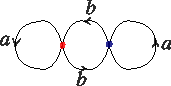
\includegraphics[]{two_s1s}\caption{\label{two_s1s}Двулистное накрытие}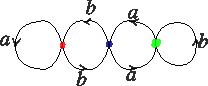
\includegraphics[]{three_s1s}\caption{\label{three_s1s}Трёхлистное накрытие}
        \end{figure}
    }
    \theorem{\label{aut_is_pi1_factor_image}\down
    \bullets{
        \item Если накрытие $p: Y \map X$ универсально, то группа автоморфизмов накрытия $\Aut(p)$ совпадает с фундаментальной группой пространства $X$.
        \item Для произвольного регулярного накрытия $\Aut(p) = \pi_1(X)/\Image(p_*)$ (факторгруппа существует, так как $\Image(p_*)$ --- нормальная подгруппа;\ это же влечёт, что $\Image(p_*)$ не зависит от выбранной точки).
    }
    \provehere{Докажем второй пункт, первый из него следует. Зафиксируем ${y_0 \in Y: p(y_0) = x_0}$.
    Определим гомоморфизм групп $\mathcal{F}: \pi_1(X) \map \Aut(p)$.

    Рассмотрим произвольную петлю $\gamma$ с концом в $x_0$.
    Её поднятие --- путь, соединяющий $y_0$ с некой точкой $y$. Так как $p(y) = x_0$, а накрытие регулярно, то найдётся автоморфизм накрытия $\tau$, такой что $\tau(y_0) = y$.
    Положим $\mathcal{F}([\gamma]) = \tau$.

    Проверим, что
    \numbers{
        \item $\mathcal{F}$ --- гомоморфизм.
        Рассмотрим петли $\gamma, \gamma'$ --- образы путей $\tilde{\gamma}$ и $\tilde{\gamma}'$, соединяющих $y_0$ с $y$ и $y'$ соответственно.
        Точкам $y$ и $y'$ соответствуют автоморфизмы $\tau$ и $\tau'$ соответственно.

        Рассмотрим путь $\tau\circ\tilde{\gamma}'$, он соединяет точку $y'$ с некой точкой, пусть это $y''$.
        Заметим, что $\mathcal{F}([\gamma] \cdot [\gamma'])$ --- это автоморфизм, переводящий $y$ в $y''$, но он же равен $\mathcal{F}([\gamma]) \cdot \mathcal{F}([\gamma']) = \tau \circ \tau'$.
        \item $\mathcal{F}$ сюръективно, так как каждой точке $y$ соответствует единственный морфизм $\tau: \tau(y_0) = y$.
        \item $\Ker(\mathcal{F}) = \Image(p_*)$, так как $[\alpha] \in \Ker(\mathcal{F}) \iff$ при поднятии $\alpha$ она не размыкается, а такие петли и составляют $\Image(p_*)$.
    }
    }
    }
    \definition[Группа $G$ действует на топологическом пространстве $X$]{
        $\exists$ гомоморфизм групп $G \map \Homeo(X)$, где $\Homeo(X)$ --- группа гомеоморфизмов пространства $X$.
    }
    Назовём эквивалентными элементы $x_1, x_2 \in X$, если $\exists g \in G: g(x_1) = x_2$.
    Так как $G$ --- группа, то эквивалентными названы элементы одной орбиты, это действительно отношение эквивалентности.
    \examples{
        \item $\R \curvearrowright S^1$ --- действие поворотами.
        \item Действие сдвигами $C_1 = \Z^2 \curvearrowright \R^2$ порождает факторпространство $\R^2/C_1 = T^2$.
    }
    \newlection{2 октября 2023 г.}
    Пусть $G \curvearrowright X$.

    \definition[Действие $G$ --- накрывающее (properly discentional action)]{
        $\forall x \in X: \exists U \ni x: \{gU\}_{g \in G}$ дизъюнктны.
    }
    \examples{
        \item Универсальное накрытие $\tilde{X} \map X$. Группа автоморфизмов накрытия действует накрывающе.
    }
    \theorem{
        Если $G \curvearrowright X$ --- накрывающее, то $p: X \map X/G$ --- накрытие.
        \provehere{
            Рассмотрим $x \in X$.
            Так как действие накрывающее, то $\exists U \ni x$, такая, что $\{gU\}_{g \in G}$ дизъюнктны.
            Тогда $p(U)$ --- правильно накрываемая окрестность.

            В самом деле, $p^{-1}(U) = \bigsqcup\limits_{g \in G}gU$.

            Осталось проверить, что $p(U)$ открыто. Это общий факт про действие групп --- образ открытого множества открыт.
            В самом деле, $p^{-1}(p(U)) = \bigcup\limits_{g \in G}gU$, что открыто, откуда $p(U)$ открыто (по определению $V$ открыто в $X/_\sim$ $\iff p^{-1}(V)$ открыто в $X$).
        }
    }
    \corollary{
        Если $X$ односвязно, то $G \sim \pi_1(X)$.
        \provehere{
            Накрытие $X \map X/G$ универсально~(\ref{aut_is_pi1_factor_image}).
        }
    }
    \theorem{
        Пусть $X$ --- хорошее пространство (существует универсальное накрытие).

        Тогда $\forall N \le \pi_1(X): \exists!$ накрытие $p: Y \map X$, такое, что $p_*(\pi_1(Y)) = N$.
        Единственность накрытия предполагается, как и следует, с точностью до изоморфизмов.
        \provehere{
            Пусть $p_0: \tilde{X} \map X$ --- универсальное накрытие.
            $G \coloneqq \pi_1(X) = \Aut(p_0)$, имеется действие $G \curvearrowright\tilde{X}, X = \tilde{X}/G$.

            Положим $Y \coloneqq \tilde{X}/N$, тогда $Y \map X$ --- накрытие с требуемой группой.
            $p_0$ пропускается через фактор.
        % https://q.uiver.app/#q=WzAsMyxbMCwwLCJcXHRpbGRle1h9Il0sWzEsMSwiWSBcXGNvbG9uZXFxIFxcdGlsZGV7WH0vTiJdLFswLDIsIlggPSBcXHRpbGRle1h9L0ciXSxbMCwyLCJwXzAiXSxbMCwxLCJwXzEiXSxbMSwyLCJcXGV4aXN0cyBwIiwwLHsic3R5bGUiOnsiYm9keSI6eyJuYW1lIjoiZGFzaGVkIn19fV1d
            \[\begin{tikzcd}[ampersand replacement=\&]
            {\tilde{X}}
                  \\
                  \& {Y \coloneqq \tilde{X}/N} \\
                  {X = \tilde{X}/G}
                  \arrow["{p_0}", from=1-1, to=3-1]
                  \arrow["{p_1}", from=1-1, to=2-2]
                  \arrow["{\exists p}", dashed, from=2-2, to=3-1]
            \end{tikzcd}\]
            Чтобы проверить, что $N = \Image(p_*)$, посмотрим, что при поднятии не размыкаются как раз петли с нужными концами.
        }
    }
    \example{
        Букет двух окружностей имеет группу $\mathcal{F}_2$. Накрытие с группой $\Z$ факторизует по одной образующей, оставляя другую. Выглядит это примерно так:~\ref{partial_factorizing}.
        \pic[0.5]{partial_factorizing}{Накрытие букета окружностей с группой $\Z$.}
    }

    \subsection{Иерархия накрытий с общей базой}
    Пусть $\pi_1(X) \ge N_1 \ge N_2$ --- цепочка вложений групп. Тогда имеется цепочка морфизмов накрытий в обратном направлении.
    % https://q.uiver.app/#q=WzAsMyxbMCwwLCJ7WH0vTl8xID0gKFlfMiwgeV8yKSJdLFswLDEsIntYfS9OXzEgID0gKFksIHlfMSkiXSxbMCwyLCJYIl0sWzAsMSwicF8yIl0sWzEsMiwicF8xIl1d
    \[\begin{tikzcd}[ampersand replacement=\&]
    {{X}/N_1 = (Y_2, y_2)}
          \\
          {{X}/N_1  = (Y, y_1)} \\
          X
          \arrow["{p_2}", from=1-1, to=2-1]
          \arrow["{p_1}", from=2-1, to=3-1]
    \end{tikzcd}\]


    \section{Фундаментальные группы клеточных пространств (CW-комплексов). Теорема Зейферта --- ван Кампена}

    \subsection{План}
    \bullets{
        \item Начинаем с одномерного остова (букета окружностей)
        \item Приклеиваем двумерные клетки, ищем соотношения
        \item Приклеиваем клетки размерности $\ge 3$, докажем, что ничего не будет меняться.
    }

    \subsection{Фундаментальная группа конечного графа}
    Пусть $X = (V, E)$ --- связный граф с $|V| = n, |E| = m$.

    Тогда $\pi_1(X)$ --- свободная группа $\mathcal{F}_{m - n + 1}$.
    \provehere{
        Выберем в графе остовное дерево $T = \left(V, \tilde{E}\right)$. $\tilde{E} = n - 1$.
        Заметим, что $(X, T)$ --- пара Борсука (клеточное пространство и подпространство).

        Стягивая $T$ в точку, получаем букет из $m - (n - 1) = m - n + 1$ окружностей.
    }

    \subsection{Теорема Зейферта --- ван Кампена}

    \subsubsection{Некоторые определения из теории групп}
    Мы будем рассматривать только конечнопорождённые конечнопредставленные группы.

    Напомним, что \textit{свободное произведение} групп $G = \angles{g_1, \dots, g_n\middle|\alpha_1, \dots, \alpha_k}$ и $H = \angles{h_1, \dots, h_m|\beta_1, \dots, \beta_l}$ --- это группа
    \[G \star H = \angles{g_1, \dots, g_n, h_1, \dots, h_m\middle|\alpha_1, \dots, \alpha_k, \beta_1, \dots, \beta_l}\]
    \examples{
        \item Свободное произведение $\Z \star \Z = \mathcal{F}_2$.
        \item <<Несвободное произведение>> $\Z \oplus \Z = \angles{a, b \middle| [a, b] = aba^{-1}b^{-1} = 1}$.
    }
    \[\text{Пусть }\begin{aligned}
                       G = &\angles{g_1, \dots, g_n\middle|\alpha_1, \dots, \alpha_k}\\ H = &\angles{h_1, \dots, h_m\middle|\beta_1, \dots, \beta_l}\\F = &\angles{f_1, \dots, f_s \middle| \gamma_1, \dots, \gamma_r}
    \end{aligned}\text{ --- группы, и зафиксированы гомоморфизмы }I: F \map G, J: F \map H.\]

    \definition[Амальгамированное произведение]{Группа
        \[G \underset{F}\star H = \angles{\arr{ccc}{g_1& \cdots& g_n\\ h_1& \cdots& h_m }\middle|\arr{ccc}{\alpha_1& \cdots& \alpha_k\\ \beta_1& \cdots& \beta_l\\ I(f_1) = J(f_1)& \cdots& I(f_s) = J(f_s)}}\]
    }

    \subsubsection{Формулировка теоремы Зейферта --- ван Кампена и доказательство для клеточных пространств}
    Пусть $X = U \cup V$, где $U, V$ --- открыты и линейно связны, $U \cap V$ линейно связно тоже.

    Выберем $x_0 \in U \cap V$, все фундаментальные группы будем рассматривать с этой отмеченной точкой.

    Имеются вложения $i: U \cap V \map U, j: U \cap V \map V$.
    Положим $I = i_*: \pi_1(U \cap V) \map \pi_1(U)$ и $J = j_*: \pi_1(U \cap V) \map \pi_1(V)$.
    \theorem[Зейферт --- ван Кампен]{
        Тогда фундаментальная группа $X$ --- это  \[\pi_1(X) = \pi_1(U) \underset{\pi_1(U \cap V)}\star \pi_1(V)\] амальгамированное произведение $\pi_1(U)$ и $\pi_1(V)$ по отношению к гомоморфизмам $I$ и $J$.
    }
    \examples[Примеры применения]{
        \item При склейке по точке никаких новых соотношений не добавляется.
        Пусть $X, Y$ --- локально односвязны.
        \[\pi_1(X \vee Y) = \pi_1(X) \star \pi_1(Y)\]
        где $\vee$ --- склейка по точке, букет.

        Для доказательства надо рассмотреть некоторую окрестность точки склейки.
        \item Например, $\pi_1(S^1 \vee S^1) = \mathcal{F}_2$.
        \item При склейке сферы из двух дисков по границе получится тривиальная группа.
        \item \textbf{23 с практики.}
        Для односвязных $A$ и $B$ и линейно связного $A \cap B$ верно, что $A \cup B$ односвязно.
        \item \textbf{24 с практики.}
        Для односвязных $A \cup B, A \cap B$ сами пространства $A, B$ тоже односвязны.
    }
    \counterexample[Важность линейной связности $U \cap V$]{
        \item При склейке двух (односвязных) отрезков по концам получится окружность с нетривиальной фундаментальной группой.
    }
    \theorem[О приклеивании двумерной клетки]{
        Пусть $Y$ --- <<хорошее>>, приклеим двумерную клетку $D^2$ по отображению $\alpha: \partial D^2 \map Y$.
        $X \coloneqq Y \sqcup_\alpha D^2$. Тогда $\pi_1(X) = \pi_1(Y)/[\alpha]^{\pi_1(Y)}$ (где $[\alpha]^{\pi_1(Y)}$ --- нормальное замыкание).
        \provehere[Доказательство из теоремы Зейферта --- ван Кампена]{
            Пусть $y \in D^2$ --- центр диска.
            Рассмотрим $U = X \sm \{y\}, V = B_{\frac{1}{2}}(y)$. Тогда пересечение $U \cap V$ гомотопически эквивалентно (внутри $U \cup V$) петле $\alpha$, $\pi_1(V) = \{e\}$.
            \[\pi_1(X) = \pi_1(Y) \underset{{[\alpha]^{\pi_1(Y)}}}\star \{e\} = \pi_1(Y)/[\alpha]^{\pi_1(Y)}\]
        }
        \provehere[Другое доказательство]{
            Пусть $\alpha: S^1 \map Y, X = Y \sqcup_{\alpha} D^2, i: Y \map X, i_*: \pi_1(Y) \map \pi_1(X)$.

            Заметим, что $i_*$ --- эпиморфизм: используя лемму о свободной точке (появлялась при доказательстве того, что на $D^n$ для $n \ge 2$ всякая петля гомотопически эквивалентна несюръективной) можно гомотопией любую петлю $\gamma: S^1 \map Y$ привести к петле $\gamma: S^1 \map X$. Для этого надо рассмотреть линейное <<отталкивание>> от данной свободной точки.

            Теперь осталось проверить, что $\Ker(i_*) = [\alpha]^{\pi_1(Y)}$.
            Очевидно включение $[\alpha] \in \Ker(i_*)$, так как ядро нормально, то $[\alpha]^{\pi_1(Y)} \le \Ker(i_*)$.

            Дальше было что-то про накрытие $Z \map Y$ с группой $[\alpha]^{\pi_1(Y)}$ и петли, которые не размыкаются при поднятии, я не понял.
        }
    }
    \newlection{9 октября 2023 г.}
    Проверим, что при приклеивании клетки размерности хотя бы 3 фундаментальная группа не меняется.
    \provehere{
        Рассмотрим склейку $X = D^n \sqcup_\phi Y$, и в ней путь $\alpha: [0, 1] \map X$.
        Берём гомоморфизм вложения $\text{in}: Y \hookrightarrow X$, индуцируем $\text{in}_*: \pi_1(Y)\map \pi_1(X)$, применяя лемму о свободной точке, находим петле в $X$ гомотопную петлю в $Y$.

        Проверим инъективность: $\alpha$ стягиваема в $X \then \alpha$ стягиваема в $Y$.
        Хотим показать, что $\exists$ гомотопия $H$, стягивающая $\alpha$.
        Для этого найдём точку в образе $D^n$, не покрываемую $H$.

        Представим $X = U \cup V$, где $U$ --- образ $B_{\frac12}(0)$, $V$ --- весь $X$ без образа $0$.
        $U \cap V = S^{n - 1} \times (0, 1)$.

        Разобьём $[0,1]\times [0,1]$ по лемме Лебега на маленькие квадратики $K_{i,j}$, так что $H(K_{i,j}) \subset U$ или $H(K_{i,j}) \subset V$.

        Обозначим $L = \bigcup\limits_{K_{i,j} \subset V}K_{i,j}$.
        Рассмотрим связные компоненты квадратиков из $L$, два квадратика будем считать связанными, если у них есть общая сторона.
        Тогда $L = \bigcup\limits_{i}L_i$, где $L_i$ --- объединение квадратиков, между любыми двумя из которых есть путь, в котором соседние квадратики имеют общую сторону.
        $\Image(\partial L_i) \subset U \cap V$.

        Можно представить $\partial L_i$, как образ $\alpha_i: S^1 \map [0,1]\times[0,1], \alpha_i(S^1) = \partial L_i$ (это правда только в том случае, если $L_i$ <<без дырок внутри>>;\ если есть дырки, то их можно заклеить квадратиками, присоединив их к $L_i$).
        Так как $S^{n-1}\times (0,1)$ односвязно, то петля $H \circ \alpha$ стягиваема в $U \cap V$.
        Тогда внутрь петли можно вклеить диск $D^2$.

        Таким образом, гомотопия не задевает образ центра шара, дальше ясно.
    }


    \section{Фундаментальные группы основных поверхностей}
    $S_p$ --- сфера с $p$ ручками, $S_q$ --- сфера с $q$ плёнками.

    Склеим сферу с $p$ ручками, как клеточное пространство.
    \[\pi_1(S_p) = \angles{a_1, \dots, a_p, b_1, \dots, b_p\middle| a_1 b_1 a_1^{-1}b_1^{-1}\dots a_p b_p a_p^{-1}b_p^{-1}}\]
    Если посчитать абелианизацию $\pi_1(S_p)$, то есть фактор по коммутанту, то будет $\underbrace{\Z \oplus \dots \Z}_{2p}$.
    \[\pi_1(S_q) = \angles{a_1, \dots, a_q \middle| a_1^2 \cdots a_q^2}\]
    Если посчитать абелианизацию $\pi_1(S_q)$, то есть фактор по коммутанту, то будет $\Z/2\Z \oplus \underbrace{\Z \oplus \dots \Z}_{q - 1}$.
    \provehere{
        В качестве базиса $\pi_1(S_q)/\sim$ можно взять $a_1 \proddots a_q$ и $a_2, \dots, a_q$.
    }
    \theorem{
        Для всякой конечнопредставленной группы $G$ $\exists$ CW-комплекс $X: \pi_1(X) = G$.
        \provehere{
            Пусть $G = \angles{a_1, \dots, a_n\middle| \alpha_1, \dots, \alpha_k}$.

            Приклеиваем клетки к букету окружностей.
        }
    }
    \corollary{
        Сферы с ручками и плёнками неэквивалентны друг другу.
    }


    \section{Построение универсального накрытия}
    \theorem{
        Для <<хороших>> пространств существует универсальное накрытие $p: \tilde{X} \map X$.
        \provehere{
            Пусть $X$ --- <<хорошее>>, то есть линейно связное, локально линейно связное, полулокально односвязное~\ref{good}.


            \bullets{
                \item Построим $\tilde{X}$, как множество.
                Выберем $x_0 \in X$, построим $\tilde{X}$. Пусть $PX = \defset{\alpha: [0, 1] \map X}{\alpha(0) = x_0}$.
                $\tilde{X} = PX/\sim$ --- пути, профакторизованные по гомотопности, связанной на концах.
                \item Определим $p: \tilde{X} \map X, p([\alpha]] = \alpha(1)$.
                \item Введём на $\tilde{X}$ топологию. Назовём $U \subset X$ хорошим, если оно открыто, линейно связно, любая петля в $U$ стягиваема в $X$.

                Введём базу топологии для $\tilde{X}$. Пусть $\alpha \in PX, \alpha(1) \in U$; обозначим через $U_{\alpha}$ класс петель вида $[\alpha s]$, где $s$ --- путь в $U$ с началом в $\alpha(1)$.

                Если $\beta \in U_{\alpha}$, то $U_{\beta} = U_{\alpha}$.
                Надо проверить включение в обе стороны. $\gamma \in U_{\alpha}, \gamma = \alpha s_1$, откуда $\gamma = \alpha s s^{-1} s_1$.

                Проверим, что $\defset{U_{\alpha}}{\alpha \in PX}$ образуют базу топологии, то есть $U_\alpha \cap V_\beta = \bigcup W_{\gamma}$.
                $\alpha(1) \in U, \beta(1) \in V$. Пусть $[\gamma] \in U_{\alpha} \cap V_{\beta}$, в частности, $\gamma(1) \in U \cap V$.
                Надо проверить, что $\gamma$ содержится в $U \cap V$ вместе с некой окрестностью.

                В качестве $W$ выберем хорошую окрестность $\gamma(1)$, содердащуюся в $U \cap V$ (достаточно выбрать линейно связную компоненту $U \cap V$).
                Достаточно проверить, что $W_{\gamma} \subset U_{\alpha}, V_{\beta}$.
                \item Докажем, что $p$ --- накрытие.
                Пусть $U \subset X$ --- хорошее. $p^{-1}(U) = \bigsqcup\limits U_{\alpha}$. В самом деле, если $U_{\alpha} \cap U_{\beta}$ непусто, то $U_{\alpha} = U_{\beta}$.

                $p^{-1}(U)$ --- классы путей с концами в $U$. $p$ непрерывно и открыто (проеряем на базе).

                Проверим, что $p\Big|_{U_\alpha}$ --- биекция. То, что это сюръекция --- очевидно, почему $p$ --- инъекция?

                Рассмотрим $[\gamma_1], [\gamma_2] \in U_{\alpha}$, предположим, что $p([\gamma_1]) = p([\gamma_2])$.
                Тогда $\gamma_1(1) = \gamma_2(1)$, и каждый из них представим в виде $alpha \cdot s$.
                Тогда пути $s_1$ и $s_2$ гомотопны, потому что окрестность хорошая, и $s_1 s_2^{-1}$ --- петля.
                \item Докажем, что $\tilde{X}$ односвязно (и линейно связно).
                Посмотрим на поднятие путей из $X$ в $\tilde{X}$.
                Выберем $\tilde{x}_0 = [\const]_{x_0} = \alpha_0$.

                $\alpha \in PX$ поднимем в $\tilde{\alpha}: [0, 1]\map\tilde{X}$. $\tilde{\alpha}(0) = \alpha_0$.
                $\tilde{\alpha}(t) \sim \alpha\Big|_{[0, t]}$.

                Таким образом, $\tilde{X}$ линейно связно.
                Проверим односвязность.

                $\tilde{\alpha}: [0,1] \map X$ --- петля. Рассмотрим проекцию $p \circ \tilde{\alpha} = \alpha$

                Докажем односвязность. $\alpha_t = \alpha(tx)$, $x \in [0, 1]$.

                Если поднятие --- петля: $[\alpha(t)] = [\const_{x_0}] = \tilde{\alpha}(0) =\tilde{\alpha}(1)$. Таким образом, $\alpha$ --- стягиваемая $\then \tilde{\alpha}$ стягиваемая.
            }
        }
    }
    Кстати, мы уже доказали, что если накрытие существует, то оно единственно.


    \chapter{Дифференциальная геометрия}
    \newlection{16 октября 2023 г.}


    \section{Дифференциальная геометрия кривых}
    \definition[Гладкая функция $f$]{Бесконечно дифференцируемая функция ${f \in C^{\infty}(\R^n \map \R^m)}$.}

    Пусть $(X, d)$ --- метрическое пространство.
    \definition[Путь (кривая)]{
        Непрерывное $\gamma: I \map X$, где $I$ --- выпуклое подмножество прямой. Чаще всего рассматривают $I = [a, b]$.
    }
    \definition[Гладкая кривая]{
        Гладкое отображение $I \map \R^n$ (все координатные отображения гладкие).
    }
    \precaution{
        Необязательно гладкое отображение выглядит гладким. График $|y| = x^{\nicefrac{3}{2}}$ представим, как гладкая кривая $\gamma(t) = (t^2, t^3)$.
    }
    \definition[Регулярная кривая]{
        Гладкая кривая $\gamma$, такая, что $\forall t: |\gamma'(t)| \ne 0$.
    }
    Пусть $\gamma_1, \gamma$ --- две кривые.
    \definition[$\gamma_1$ --- перепараметризация $\gamma$]{
        $\exists$ строго возрастающее $\phi$: $\gamma_1 = \gamma \circ \phi$.
    }
    Для гладких кривых вводят \textit{гладкую перепараметризацию} $\phi \in C^{\infty}$, $\phi' > 0$.
    \definition[Кривые $\gamma_1, \gamma_2$ эквивалентны]{
        Существует перепараметризация $\phi$.
        Пишут $\gamma_1 \sim \gamma_2$
    }
    \fact{
        Эквивалентность кривых --- отношение эквивалентности.
        Аналогичный факт верен для эквивалентности гладких перепараметрищаций гладких кривых.
    }
    \begin{definition_env}
        Разбиение отрезка $[a, b]$
    \end{definition_env}{
        Разбиение $a = t_0 \le \cdots \le t_k = b$.
    }
    \begin{definition_env}
        Длина кривой $\gamma: [a, b] \map X$
    \end{definition_env}{
        $L(\gamma) \bydef \sup\limits_{a = t_0 \le \cdots \le t_k = b} \sum\limits_{i = 0}^{k-1}d(\gamma(t_i), \gamma(t_{i + 1}))$
    }
    \note{
        Согласно неравенству треугольника, при измельчении разбиения $\sum\limits_{i = 0}^{k-1}d(\gamma(t_i), \gamma(t_{i + 1}))$ возрастает.
    }
    \definition[Кривая спрямляемая]{$L(\gamma) < \infty$}
    \example{
        Неспрямляемую кривую придумать несложно.
        Например, соединим ломаной соседние точки в последовательности $(\alpha_n, (-1)^n\beta_n)$, где $\alpha_n, \beta_n$ --- убывающие, стремящиеся к нулю, последовательности, причём $\sum\limits_{n \ge 0}\beta_n = \infty$.
    }
    \proposal{
        $\gamma_1 \sim \gamma_2 \then L(\gamma_1) = L(\gamma_2)$.
    }
    \statement{
        Если кривая $\gamma$ гладкая, то $L(\gamma) = \int\limits_{a}^{b}|\gamma'(t)|\d t$.
        \provehere{
            Докажем неравенство в обе стороны.
            \bullets{
                \item $\int\limits_{a}^{b}|\gamma'(t)|\d t \le L(\gamma)$.

                $\gamma'$ равномерно непрерывна. Таким образом, $\forall \eps > 0: \exists \delta > 0: |t_1 - t_2| \le \delta \then |\gamma'(t_1) - \gamma'(t_2)| < \eps$.
                Разобьём отрезок на $\ceilfrac{b - a}{\delta}$ частей равной длины (каждая часть имеет длины не больше $\delta$) точками $a = t_0 \le \cdots \le t_k = b$.
                Тогда \[(1 - \eps)\int\limits_{t_i}^{t_{i + 1}}|\gamma'(t)|\d t\: \le\: \abs{\gamma(t_i) - \gamma(t_{i + 1})}\]
                откуда $(1 - \eps)\int\limits_{a}^{b}|\gamma'(t)|\d t \le L(\gamma)$. Устремим $\eps \to 0$.
                \item $L(\gamma) \le \int\limits_{a}^{b}|\gamma'(t)|\d t$.

                Рассмотрим разбиение $a = t_0 \le \cdots \le t_k = b$.
                Используем неравенство \[|\gamma(t_{i + 1}) - \gamma(t_i)| = \abs{\int\limits_{t_i}^{t_{i + 1}}\gamma'(t)\d t} \le \int\limits_{t_i}^{t_{i + 1}}\abs{\gamma'(t)}\d t\]
            }
        }
    }
    \corollary{
        $\int\limits_{a}^{b}|\gamma'(t)| \d t$ не зависит от перепараметризации.
    }
    \theorem{
        Отрезки в $\R^n$ кратчайшие.
        Иными словами, $\forall r, s \in \R^n$ отрезок \begin{align*}
                                                           \alpha: [0, 1] &\map \R^n\\t &\mapsto r + t(s - r)
        \end{align*}
        имеет наименьшую длину среди всех кривых (необязательно гладких), соединяющих $r$ и $s$.
        \provehere{
            Рассмотрим путь $\gamma$, соединяющий $r$ и $s$.
            Рассмотрим разбиение $a = t_0 \le t_1 = b$.
            По определению $L(\gamma) \ge \abs{\gamma(b) - \gamma(a)}$.
        }
    }
    \theorem{
        Кратчайшие пути на сфере $S^2$ --- дуги больших кругов.
        \provehere{
            Покажем, что $\forall \gamma: [a, b] \map S^2: L(\gamma) \ge \angle(\gamma(a), \gamma(b))$.
            Выберем $\eps > 0$, из равномерной непрерывности $\gamma$ найдётся $\delta > 0: |t_1 - t_2| \le \delta \then \abs{\gamma(t_1)  - \gamma(t_2)} < \eps$.

            Рассмотрим разбиение $a = t_0 \le \cdots \le t_k = b$, такое, что $\abs{t_{i + 1} - t_i} \le \eps$.

            \[L(\gamma) \ge \sum\limits_{i = 0}^{k - 1}|\gamma(t_i) - \gamma(t_{i + 1})| \ge \sum\limits_{i = 0}^{k - 1}\angle(\gamma(t_i), \gamma(t_{i + 1}))\cdot\frac{\eps}{2\arcsin\left(\nicefrac{\eps}{2}\right)} \ge \angle(\gamma(a), \gamma(b)) \cdot \frac{\eps}{2\arcsin\left(\nicefrac{\eps}{2}\right)}\]
            Устремляем $\eps \to 0$.
        }
    }

    \subsection{Параметризация кривой длиной дуги}
    Пусть $\gamma: [a, b] \map X$, где $(X, d)$ --- метрическое пространство.
    \definition[Натуральная параметризация]{
        $L\left(\gamma\Big|_{[t_1, t_2]}\right) = t_1 - t_2$
    }
    \statement{
        Гладкая кривая параметризована натурально $\iff \abs{\gamma'} \equiv 1$.
        \provewthen{
            Если $\exists t_0: \gamma'(t_0) = 1 + \delta$, то $\exists \eps > 0: |t - t_0| < \eps \then |\gamma'(t)| - |\gamma'(t_0)| \le \frac{\delta}{2}$.
            Тогда так как длина --- интеграл модуля производной, то в $\eps$-окрестности $t_0$ не выполняется определение натуральной параметризации.
        }{
            Длина --- интеграл модуля производной.
        }
    }
    \theorem{
        Для любой регулярной кривой существует натуральная параметризация.
        Эта параметризация единственна с точностью до сдвига на константу: если $\gamma: [a, b] \map X$ --- натуральная параметризация, то \begin{align*}
                                                                                                                                               \tilde{\gamma}: [a + c, b + c] &\map X\\t + c &\mapsto \gamma(t)
        \end{align*} тоже.
        \provehere{
            Пусть $\gamma: [a, b] \map \R^n$.

            Эта параметризация устроена так: $s: [a, b] \map [0, L(\gamma)] \qquad s(t) = L\left(\gamma\Big|_{[a, t]}\right) = \int\limits_{a}^{t}|\gamma'(t)|\d t$.
            \[s'(t) = |\gamma'(t)| > 0,\text{ поэтому $s$ --- валидная перепараметризация.}\]
            Положим $\gamma_1 = \gamma \circ s^{-1}$.
            \[\gamma_1' = (\gamma \circ (s^{-1}))' = \gamma' \cdot \frac{1}{s'} \quad \then \quad |\gamma_1'| = \frac{|\gamma'|}{|\gamma'|} = 1\]
            Если же есть две перепараметризации $\gamma_1$, $\gamma_2$, то $|\gamma_1'| = |\gamma_2'| \cdot |\phi'|$, откуда $|\phi'| = 1$, то есть используя $\phi' > 0$ (получаем, что $\phi$ --- сдвиг на константу)
        }
    }
    \statement{
        Пусть $A: I \map \R^n, B: I \map \R^m$; пусть $*: \R^n \times \R^m \map \R^k$ --- билинейно.
        Тогда у отображения $A * B: I \map \R^k$ производная считается по правилу
        \[(A * B)' = A' * B + A * B'\]
        \provehere{

        }
    }
    \examples{
        \item В качестве $*$ может выступать скалярное произведение, векторное произведение, умножение вектора на число (и вообще умножение матриц)\ldots
    }


    \section{Кривизна плоской кривой, базис Френе}
    Далее везде считаем, что кривая $\gamma: [a, b] \map \R^2$ параметризована натурально, то есть $|\gamma'| = 1$.
    Будем обозначать $v = \overrightarrow{v} = \gamma'$ --- вектор скорости.
    \definition[Базис Френе]{
        Пара $(v, n)$, такая, что $v \perp n$, причём $(v, n)$ --- правый ортонормированный базис.
        Данный вектор $n$ --- \textit{нормаль к плоской кривой}.
    }
    Так как $\angles{v, v} = 1$, то $\angles{v', v} = 0$, откуда $v' \perp v$ и $\exists! \kappa(t) \in \R: v' = \kappa n$.
    \definition[Кривизна плоской кривой]{
        Данное число $\kappa$.
    }

    \subsection{Формулы Френе}
    \bullets{
        \item По определению кривизны $v' = \kappa n$
        \item $\angles{n, v} = 0$, откуда $\angles{n', v} + \angles{n, v'} = 0$, откуда $n' = -\kappa v$.
    }
    \newlection{23 октября 2023 г.}

    \statement{
        Длина полунепрерывна снизу.
        Пусть $\gamma_n$ --- последовательность кривых: $\gamma_n: [0, 1] \map \R^2$, таких, что $\gamma_n(t) \underset{n \to \infty}\Map \gamma_{\infty}(t)$.

        Тогда $l(\gamma_\infty) \le \varliminf\limits_{n \to \infty} l(\gamma_n)$.
        \provehere{
            Рассмотрим $\eps > 0$. Для него найдётся последовательность точек $0 = t_0 \le \cdots \le t_k = 1: \sum\limits_{i = 0}^{k - 1}|\gamma_{\infty}(t_{i+1})-\gamma_{\infty}(t_i)| \ge l(\gamma_{\infty}) - \eps$.

            Выберем настолько большой номер $m: \forall i: \abs{\gamma_m(t_i) - \gamma_{\infty}(t_i)} < \frac{\eps}{m}$. Тогда $l(\gamma_m) \ge l(\gamma_{\infty}) - 3\eps$.

            Устремляя $\eps \to 0$, получаем искомое утверждение.
        }
    }
    \note{
        $\kappa$ --- кривизна двумерной кривой (кривизна со знаком).

        Если же работать в более, чем двумерном пространстве, то у кривизны не будет знака. Там
        \[v \coloneqq \gamma' \quad N = \frac{\gamma''}{|\gamma''|}\]
        Так как $\angles{\gamma',\gamma'} = 1$, то $\angles{\gamma'', \gamma'} = 0$.

        Кривизна без знака $k \coloneqq |\gamma''|$.
    }
    Пусть $\gamma: I \map \R^n$ --- регулярная кривая, $M \subset \R^n$ --- множество.
    \definition[$\gamma$ имеет порядок касания не меньше $m$ со множеством $M$ в точке $t_0$]{
        $d(\gamma(t), M) = o((t-t_0)^k)$.
    }
    Если две регулярные кривые можно параметризовать так, что $\gamma_1^{(i)} = \gamma_2^{(i)}$ для $i \le m$, то порядок касания не меньше $m$.
    \definition[Касательная прямая к $\gamma$ в точке $t_0$]{
        Кривая, проходящая через $\gamma(t_0)$ с направляющим вектором $\gamma'(t_0)$.
    }
    \proposal{
        Порядок касания касательной и кривой не меньше 1.
    }
    \fact{
        Кривизна окружности радиуса $R$ --- это $\pm \frac1R$.
    }
    Пусть $\gamma$ --- регулярная кривая $\gamma(t_0) = \gamma_0$.
    \definition[Соприкасающаяся окружность к $\gamma$ в точке $t_0$]{
        Окружность радиуса $\abs{\frac1\kappa}$ с центром $\gamma_0 + \frac{n}{\kappa}$. (или минус?)
    }
    Разложив в ряд Тейлора, можно показать, что порядок касания соприкасающейся окружности $\ge 2$.
    \theorem{
        Пусть $\gamma$ --- регулярная кривая. Тогда кривизна считается по формуле $\kappa(t_0) = \frac{[\gamma'(t_0), \gamma''(t_0)]}{|\gamma'(t_0)|^3}$.
        Здесь $[x, y]$ --- смешанное или внешнее произведение $x$ и $y$
        \provehere{
            Перепараметризуем $\gamma$ натуральной параметризацией $\gamma = \overline{\gamma}(\phi(t))$.
            Тогда $|\gamma'| = \phi'$, $\gamma' = \phi' v$ и \[\gamma'' = \phi'' \cdot \overline{\gamma}' + (\phi')^2 \cdot \overline{\gamma}'' = \phi'' \cdot \overline{\gamma}' + |\gamma'|^2 \cdot \kappa n\]
            Отсюда получаем $[\gamma', \gamma''] = [|\gamma'|^2, |\gamma'|^2 \kappa n] = |\gamma'|^3 \cdot \kappa$
        }
    }

    \subsection{Поворот кривой}
    Всякое отображение $f: [a, b] \map S^1$ поднимается до отображения $\alpha: [a, b] \map \R$, такого, что $p \circ \alpha = f$.
    % https://q.uiver.app/#q=WzAsMyxbMCwxLCJbYSwgYl0iXSxbMSwxLCJTXjEiXSxbMSwwLCJcXFIiXSxbMiwxLCJwIl0sWzAsMSwiZiIsMl0sWzAsMiwiXFxhbHBoYSIsMCx7InN0eWxlIjp7ImJvZHkiOnsibmFtZSI6ImRhc2hlZCJ9fX1dXQ==
    \[\begin{tikzcd}[ampersand replacement=\&]
          \& \R \\
          {[a, b]} \& {S^1}
          \arrow["p", from=1-2, to=2-2]
          \arrow["f"', from=2-1, to=2-2]
          \arrow["\alpha", dashed, from=2-1, to=1-2]
    \end{tikzcd}\]
    Если $f$ гладкое, то $\alpha$ гладкое --- выражается где-то как арксинус, где-то --- как арккосинус.

    В дальнейшем мы часто будем поднимать вектор скорости $\gamma'$, если $\gamma$ --- кривая при $|\gamma'| = 1$..

    \definition[Поворот плоской кривой]{
        $\int\limits_{a}^{b}\kappa(t)\d t$, где $\kappa(t)$ --- кривизна в натуральной параметризации.
    }
    \theorem{
        Пусть $\gamma$ --- натуральная параметризация, $v$ --- вектор скорости. Пусть $\alpha(t)$ --- непрерывный аргумент (полученный из поднятия), такой, что $v(t) = (\cos(\alpha(t)), \sin(\alpha(t)))$.
        Тогда $\alpha' = k$ и $\int\limits_{a}^{b}\kappa(t)\d t = \alpha(b) - \alpha(a)$.
        \provehere{
            $\kappa n = v' = (-\sin(\alpha), \cos(\alpha)) \cdot \alpha'$. Можно проверить, что $(-\sin(\alpha), \cos(\alpha)) \perp (\sin(\alpha), \cos(\alpha))$, причём векторы образуют правый базис.
        }
    }
    \theorem{
        Для любой гладкой функции $\tilde{\kappa}: I \map \R$: $\exists! \gamma: I \map \R^2$ --- натурально параметризованная кривая, такая, что $\kappa_\gamma = \tilde{\kappa}$. Единственность предполагается с точностью до движения, сохраняющего ориентацию.
        \provehere{
            Имеет место даже более точное утверждение: при заданном $\tilde{\kappa}$: $\forall p0, v_0$: $\exists!$ натурально параметризованная кривая $\gamma: \gamma(a) = p_0, \gamma'(a) = v_0$.

            Для любой пары векторов одной длины существует единственное движение, сохраняющее ориентацию, переводящее точку в точку, вектор в вектор.

            Пусть $\gamma$ --- натурально параметризована, $v = (\cos\alpha, \sin\alpha)$. $\dot{\alpha} = \tilde{\kappa}$, причём $\alpha$ определяется единственным образом с точностью до константы $2\pi$.
            \[\alpha = \alpha_0 + \int\limits_{a}^{b}\tilde{\kappa}(\tau)\d \tau\]
            В качестве $\alpha_0$ можно выбрать угол, который составляет $v_0$ с осью абсцисс.
            \[\gamma(t) = \int\limits_{a}^{t}v(\tau)\d \tau + c_0\text{, где $c_0 = p_0, v(\tau) = (\cos\alpha, \sin\alpha)$.}\]
            Это построение одновременно показывает существование и единственность искомой кривой $\gamma$.
        }
    }

    \subsection{Замкнутые кривые}
    Пусть $\gamma: [a, b] \map \R^2$.
    \definition[Кривая $\gamma$ замкнута]{ Функцию $\gamma$ можно продолжить до периодической с периодом $b - a$.
    Иными словами, $\gamma^{(i)}(a) = \gamma^{(i)}(b)$ для $i \in \N_0$.}

    \definition[Простая кривая $\gamma$]{
        Кривая без самопересечений.
    }
    Поворот замкнутой кривой --- $2\pi n$, $n \in \Z$.
    \theorem{
        Поворот простой замкнутой кривой --- $\pm 2\pi$.
        \provehere{
            Пусть $\gamma: [0, L] \map \R^2$ параметризована натурально.
            Выберем базис так, что $\gamma(0) = (0, 0)$.
            Сдвинем аргумент так, что $\gamma(t) = (x, y)$, причём $y \ge 0$ для всех $t$.

            Из гладкости сразу получается $\gamma'(0) = (1, 0)$.

            Пусть $T = \defset{(t,\tau) \subset\R^2}{0 \le t \le \tau \le L}$.
            Устроим $\mathcal{F}: \arr{ccc}{T &\map& S^1\\(t, \tau)&\mapsto&\frac{\gamma(\tau) - \gamma(t)}{|\gamma(\tau) - \gamma(t)|}}$.
            Если же $t = \tau$, то дооопределим $\mathcal{F}$ по непрерывности: $\mathcal{F}(t,t) = \gamma'(t)$.

            $T$ односвязно, поэтому существует поднятие --- непрерывный аргумент $A$: $\mathcal{F}(t,\tau) = \sin(A(t,\tau)), \cos(A(t,\tau))$.
        % https://q.uiver.app/#q=WzAsMyxbMCwxLCJUIl0sWzEsMCwiXFxSIl0sWzEsMSwiU14xIl0sWzAsMiwiXFxtYXRoY2Fse0Z9Il0sWzAsMSwiQSIsMCx7InN0eWxlIjp7ImJvZHkiOnsibmFtZSI6ImRhc2hlZCJ9fX1dLFsxLDIsInAiXV0=
            \[\begin{tikzcd}[ampersand replacement=\&]
                  \& \R \\
                  T \& {S^1}
                  \arrow["{\mathcal{F}}", from=2-1, to=2-2]
                  \arrow["A", dashed, from=2-1, to=1-2]
                  \arrow["p", from=1-2, to=2-2]
            \end{tikzcd}\]
            Так как $A(t,t)$ --- непрерывный аргумент для $\gamma'(t) = \mathcal{F}(t,t)$, то поворот кривой $\gamma$ --- разность $A(L,L) - A(0,0)$.
            \[A(L,L) - A(0,0) = (A(L,L) - A(0,L)) + (A(0,L) - A(0,0))\]
            Если посмотреть на $A\Big|_{\{0\}\times[0,L]}$, то окажется, что это векторы с фиксированным началом, которые всегд смотрят в верхнюю полуплоскость.
            Из существования непрерывного аргумента $A(0,t) \in [0, \pi]$ и $A(0,L) - A(0,0) = \pi - 0 = \pi$

            При подсчёте $A(L,L) - A(0,L)$ будет то же, только аргумент меняется в пределах $[-\pi, 0]$.
            Разность опять выйдет $\pi$, итого $A(L,L)-A(0,0) = 2\pi$.
        }
    }

    \subsection{Выпуклые кривые на плоскости}
    Пусть $\gamma$ --- замкнутая гладкая регулярная кривая.

    Дадим два определения, и покажем их равносильность.
    \definition[Выпуклая кривая, 1]{
        Простая кривая, обходящая границу выпуклого компакта $K$: $\Image(\gamma) = \partial(K)$.
    }
    \definition[Выпуклая кривая, 2]{
        Кривая, лежащая по одну сторону от любой своей касательной.
    }
    \fact{
        Эти определения равносильны.
        \provetwhen {
            Касательная к $\gamma$ в точке $t$ --- опорная прямая для компакта.
            Значит, она лежит только по то сторону от своей касательной, в которую лежит компакт.
        }{
            Рассмотрим $K \coloneqq \text{conv}(\Image(\gamma))$. $\nexists t_0: \gamma(t_0)$ --- внутренняя точка $K$.

            Так как $K$ гомеоморфно диску $D^2$, то $\partial K \sim S^1$, $\Image(\gamma) \sim S^1$.
            При этом $\gamma \subset \partial K$ --- простая кривая без самопересечений.

            Несложно показать, что инъективное непрерывное отображение $S^1 \map S^1$ --- гомеоморфизм.
        }
    }
    \theorem{
        Следующие условия равносильны:
        \numbers{
            \item $\gamma$ выпукла
            \item $K_\gamma$ не меняет знак (всегда $\ge 0$ или всегда $\le 0$).
            \item Для любой прямой $L: \exist$ ровно две касательные к $\gamma$, параллельные $L$.
            \provehere{\down
            \bullets{
                \item[$1 \then 2$] Выберем какую-то ориентацию, зафиксируем $t_0$.
                Покажем, что если $\gamma$ лежит слева от касательной в $t_0$, то кривизна $\ge 0$, если $\gamma$ лежит справа от касательной в $t_0$, то кривизна $\le 0$.

                Пусть $\delta: [a, b] \map \{\pm 1\}$ --- определяет, лежит кривая слева или справа от прямой.
                Покажем, что $\delta$ непрерывно, эквивалентно, локально постоянна.

                Выберем точку $q: \angles{\overrightarrow{\gamma(t_0) q}, n} > 0$.
                Тогда в некоторой окрестности $t_0:$  $\angles{\overrightarrow{\gamma(t) q}, n} > 0$ тоже.
            }
            }
        }
    }
    \newlection{30 октября 2023 г.}
    //todo
    \newlection{6 ноября 2023 г.}


    \section{Базис Френе и кривизны в $\R^n$}
    Пусть $\gamma: I \map \R^n$ --- невырожденная кривая в $\R^n: \gamma', \dots, \gamma^{(n - 1)}$ линейно независимы.
    \theorem{
        Пусть $\gamma$ --- натурально параметризованная невырожденная кривая в $\R^n$.
        Тогда $\exists v_1, \dots, v_n: I \map \R^n$ --- базис Френе, зависящий от времени, и $\exists!$ гладкие функции $k_1, \dots, k_{n-1}: I \map \R^n$, такие, что $k_1, \dots, k_{n-2} > 0, k_{n-1}$ имеет любой знак.
        При этом выполнены формулы Френе
        \numbers{
            \item $\gamma'(t) = v_1(t)$
            \item $\all{v_1' = k_1 v_2 \\ v_i' =  -k_{i-1}v_{i-1} + k_i v_{i+1} \\ v_n' = -k_{n-1}v_{n-1}}$.
            Это также можно записать в виде $v' = Kv$, где $K$ --- матрица из кривизн.
            \item Базис $v_1, \dots, v_n$ --- правый ортонормированный.
        }
        \provehere{
            $|\gamma'| = 1$. Положим $v_1 \coloneqq \gamma'$.

            Рассматриваем набор производных $\gamma', \dots, \gamma^{(n-1)}$, по ним строится $v_1, \dots, v_{n-1}$ при помощи ортогонализации Грама --- Шмидта.
            Алгоритм возвращает ортонормированный базис какой-то гиперплоскости коразмерности 1, он единственным образом дополняется до ортонормированного правого базиса $\R^n$.

            Дальше по данному базису раскладываются вектора производных.
            Проверим, что соответствующие коэффициенты получаются нужного знака, и много кто --- нули: проверим соответствие (2).
            \[v_i' = c_{i,1}v_1 + \cdots + c_{i,n}v_n\]
            Так как $\angles{v_i,v_i} = 1$, то $\angles{v_i',v_i} = 0$. Так как $\angles{v_i,v_j} = 0$, то $\angles{v_i',v_j} = -\angles{v_i,v_j'}$.
            Таким образом, матрица $(c_{i,j})$ кососимметричная.
            $v_i \in \Lin(\gamma^{(1)}, \dots, \gamma^{(i)})$, откуда $v_i' \in \Lin(\gamma^{(1)},\dots,\gamma^{(i+1)}) = \Lin(v_1, \dots, v_{i +1})$. Согласно кососимметричности видим, что почти нужные коэффииценты равны нулю.

            Проверить положительность кривизн $k_1, \dots, k_{n-2}$, на лекции сделать не вышло.
%            По построению базиса Френе $\angles{\gamma^{(i)}, v_i} > 0$.
%            Что дальше --- загадка.

            Проверим однозначность определения базиса Френе. Пойдём индукцией: пусть $v_1, \dots, v_{i}$ однозначно определены. Почему $v_{i+1}$ однозначно определён?
            Из формул $v_{i+1} \perp \Lin(v_1, \dots, v_{i})$, $v_i' \in \Lin(v_1, \dots, v_{i+1})$. Производная $v_i'$ определена однозначно, значит, $\Lin(v_1, \dots, v_{i+1})$. определена, как $\Lin(v_1, \dots, v_i, v_i')$.
            Так как $k_i = \angles{v_i', v_{i+1}} > 0$, то направление $v_{i+1}$ определено однозначно. $v_n$ же определяется однозначно из того, что базис --- правый.
        }
    }
    \theorem{
        Пусть даны гладкие функции $k_1, \dots, k_{n-1}: I \map \R$, такие, что $k_1, \dots, k_{n-2} \ge 0$.
        Тогда существует (и единственна с точностью до движения) кривая с такими кривизнами.
        \provehere{
            Отметим произвольную точку, произвольно выберем правый ортонормированный базис $v_0 = v(0), v_1, \dots, v_{n-1}$.
            В матричной записи $v' = Kv$. Это линейное дифференциальное уравнение, имеет единственное решение при начальных данных $v_0, \dots, v_{n-1}$.

            Таким образом ищется функция $v(t)$, тогда $\gamma = p_0 + \int\limits_{t_0}^{t}v(\tau)\d \tau$.

            Заметим, что $(v^tv)' = (v')^t v + v^t v' = v^t K^t v + v^t K v = v^t\underbrace{(K^t + K)}_{0}v = 0$, откуда базис $v$ --- правый ортонормированный в любой момент времени, а не только в нулевой.
        }
    }


    \section{2-мерные поверхности в $\R^3$}
    Далее всё происходит в $\R^2$
    \definition[Топологическая поверхность $\Sigma$]{
        Подмножество $\Sigma \subset \R^3$, которое может быть получено, как образ топологического вложения связного двумерного многообразия $f: M \hookrightarrow \R^3$.

        Топологичность вложения означает, что топология, индуцируемая с помощью $f$ топологией $\R^3$ совпадает с собственной топологией $M$.
    }
    \definition[Гладкая поверхность $\Sigma \subset \R^3$] {
        Поверхность $\Sigma$, которая локально может быть представлена, как график гладкой функции: $\forall p \in M$: можно ввести координатные оси $x,y,z$ с нулём в $p$, так, что $\exists \underset{\ni p}{U} \subset \R^3: \exists f: (\Omega \subset \R^2_{x,y})\underset{\text{гладко}}\map \R: \Sigma \cap U = \Gamma_f$ (здесь $\Gamma_f$ --- график $f$ в $\R^3_{x,y,z}$).
    }
    \definition[Регулярное отображение $r$]{
        Дифференциал $\d r$ невырожден.
    }
    Невырожденность гладкого $r: \R^2 \map \R^3$ при введении базиса $(u, v)$ в $\R^2$ можно переформулировать так: $\der{r}{u} \times \der{r}{v} \ne 0$.

    \subsection{Локальная параметризация}
    \theorem{\label{regular-param-sigma}
    Пусть $\Omega \subset \R^2$, пусть $r: \Omega \map \R^3$ --- регулярное (всегда подразумевается, что ещё и гладкое).
    Если $r: \Omega \map \R^3$ --- вложение, то $r(\Omega) \eqqcolon \Sigma$ --- гладкая поверхность.
    \provehere{
        Рассмотрим $z$ покоординатно: \[(u, v) \overset{r}\mapsto \vect{r_1(u, v) = x(u,v)\\r_2(u,v) =y(u,v)\\r_3(u,v)=z(u,v)}\]
        Условие невырожденности дифференциала: $\abs{\arr{cc}{x_u & y_u \\ x_v & y_v}} \ne 0$, здесь $x_u$ --- частная производная (?).

        Пусть $p = r(x_0)$. Из невырожденности дифференциала $\exist W \subset \Lin(x, y), V \subset \Lin(u, v)$ и обратное отображение $s: W \map V$, такое, что $(r_1, r_2) \circ s = \id$.
        Тогда $(r \circ s)(x, y) = (x, y, (r_3 \circ s)(x, y))$.
        Обозначим $f \coloneqq r_3 \circ s$; заметим, что $r(V)$ открыто в $\Sigma$, получаем, что $r(V)$ переписывается в виде $\Sigma \cap U$ для некоторого открытого $U \subset \R^3$.
    }
    }
    \definition[Регулярная параметризация поверхности $\Sigma$]{Отображение $r$, как в~(\ref{regular-param-sigma})}
    \note{
        Далеко не всякая поверхность в $\R^3$ гомеоморфна плоскости, например, у сферы $S^2 \subset \R^3$ нет регулярной параметризации.

        Тем не менее, существует локальная регулярная параметризация, которая получается из тех же соображений, что в теореме.
    }
    Пусть $r$ --- регулярная параметризация, как в теореме.
    Тогда $\exists r^{-1} \eqqcolon \phi: \Sigma \map \Omega$, оно называется \textit{картой}.

    \definition[Две регулярные параметризации $r_1: \Omega_1 \map \Sigma$ и $r_2: \Omega_2 \map \Sigma$]{
        $\exists$ гладкое регулярное $s: \Omega_1 \map \Omega_2$, такое, что $s^{-1}$ --- тоже гладкое регулярное, такое, что $r_1 = r_2 \circ s$
    }
    \excersice{
        Для гладкой поверхности локально любые две параметризации эквивалентны.
    }
    Пусть $r: \Omega \map \Sigma$ --- регулярная параметризация.

    \indent{Пусть $l(t) = (t, \const)$ --- путь, обозначим данную константу $v_0$.
    Можно ввести координатные линии $r(t, v_0)$ и $r(u_0, t)$.

    Векторы скорости координатных линий $r_u(t, v_0)$ и $r_v(u_0, t)$.

    Пусть $\tilde{\gamma} = r \circ \gamma$. $\gamma$ регулярна $\iff$ $\tilde{\gamma}$ регулярна.
    Обратно можно получить $\gamma = \phi \circ \tilde{\gamma}$.
    }
    \statement{Пусть $F: \R^m \map \R^n$ --- гладкое отображение.

    Чтобы посчитать производную по направлению $v$, можно взять произвольную гладкую кривую $\gamma$, такую, что $\gamma(0) = x, \gamma'(0) = v$, тогда $(f \circ \gamma)$ --- искомая.
    }
    \definition[Касательное пространство к $\Sigma$ в точке $p = r(x)$]{
        $T_p(\Sigma) = \d_x r(\R^2)$.
    }
    Касательное пространство можно рассматривать, как линейное пространство, или аффинное пространство в $\R^3$.

    \statement{
        Касательное пространство не зависит от параметризации.
        \provehere{
            Можно определить эквивалентным образом: касательное пространство $T_p(\Sigma) = \{\text{векторы скорости гладких кривых, проходящих через точку $p$}\}$
        }
    }
    Касательная плоскость --- линейное пространство, натянутое на векторы $\der{r}{u}$ И $\der{r}{v}$ --- стандартный базис в касательном пространстве.
    $\der{r}{u} = r_u = \d r(1, 0), \der{r}{v} = r_v = \d r(0, 1)$.
    \newlection{13 ноября 2023 г.}
    \subsection{Гладкие функции на поверхности}
    Определим гладкую функцию $f: \Sigma \map \R$ из поверхности в прямую.
    \definition[Функция $f$ гладкая]{
    $\forall p \in \Sigma: \exists U \ni p$ --- карта, такая, что $f$ --- гладкая в карте $U$, то есть $\exists r: \Omega \map U: f \circ r$ --- гладкая.
    }
    \statement{
    Условие гладкости $f: \Sigma \map \R$ равносильно следующим:
    \numbers{
    \item $f$ гладкая в любой карте.
        \item $\exists F: (\subset \R^3) \map \R$ --- продолжение $f$, гладкое в окрестности любой точки.
    \provehere{
    \numbers{
        \item Отображение перехода между картами $s$ --- регулярно, и $s^{-1}$ --- тоже регулярно.
    \note{
Из теоремы об обратном отображении $s$ --- регулярная биекция.
    }
    \item Если поверхность локально задаётся графиком $\Sigma = (x, y, h(x, y))$, то можно определить $F(x, y, z) = f(x, y, h(x, y))$.
    }
    }
    }
    }
    \subsection{Производная по направлению}
    Пусть $p \in \Sigma, X \in T_p(X)$.

    Пусть $f: \Sigma \map \R$ --- гладкая функция, пусть $\tilde{\gamma}: (-e\sp, +\eps) \map \Sigma$ --- кривая на поверхности.
    Пусть $p \coloneqq \tilde{\gamma}(0), \tilde{\gamma}'(0) = X$.
    Тогда
    \numbers{
    \item $(f \circ \tilde{\gamma})$ --- гладкая.
    \item Для всякой параметризации $r: \Omega \map \R^3$: $(f \circ \tilde{\gamma})'(0)$ --- не зависит от $\tilde{\gamma}$.
    \item Для всякой параметризации $r: \Omega \map \R^3$: $(f \circ \tilde{\gamma})'(0) = X_1 \der{f \circ r}{u} + X_2 \der{f \circ r}{v}$.
    }
    \provehere{
        1. $f \circ \tilde{\gamma} = f \circ r \circ \gamma$
    3. Пусть $\gamma = (u(t), v(t))$. $(f \circ r \circ \gamma)' = (f \circ r)'_u \cdot u' + (f \circ r)'_v \cdot v'$. $\gamma'(0) = (X_1, X_2)$.

    }
    $X_1 (f \circ r)'_u + X_2 (f \circ r)'_v$ называется производной функции $f$ по направлению $X$, обозначается $X(f)$.

    \definition[$f: \Sigma \map \R^3$ --- гладкая функция]{
    $f$ --- гладкая покоординатно.
    }
    Пусть теперь есть две поверхности $\Sigma_1$ и $\Sigma_2$.

    Если $\Image(\tilde{f}) \subset \Sigma_2$, то $\tilde{f}$ --- гладкая функция $\Sigma_1 \map \Sigma_2$ из одной поверхности в другую.

    Можно рассмотреть соответствующую $\tilde{f}: \Sigma_1 \map \Sigma_2$
    % https://q.uiver.app/#q=WzAsNCxbMCwxLCJcXE9tZWdhXzEiXSxbMCwwLCJcXFNpZ21hXzEiXSxbMSwwLCJcXFNpZ21hXzIiXSxbMSwxLCJcXE9tZWdhXzIiXSxbMCwzLCJmIiwyXSxbMCwxLCJyXzEiLDJdLFsxLDIsIlxcdGlsZGV7Zn0iLDJdLFszLDIsInJfMiJdXQ==
    \[\begin{tikzcd}[ampersand replacement=\&]
    {\Sigma_1} \& {\Sigma_2} \\
    {\Omega_1} \& {\Omega_2}
    \arrow["f"', from=2-1, to=2-2]
    \arrow["{r_1}"', from=2-1, to=1-1]
    \arrow["{\tilde{f}}"', from=1-1, to=1-2]
    \arrow["{r_2}", from=2-2, to=1-2]
    \end{tikzcd}\]
    \statement{$\tilde{f}$ --- гладкая $\iff f$ гладкая в любой карте.
    \provehere{
    \bullets{
    \item[$\then$] Рассмотрим хорошую карту $\Sigma = \Gamma_h: r: (x, y) \mapsto (x, y, h(x, y))$.
    \item[$\when$] Посмотреть на коммутативную диаграмму.
    }
    }
    }
    Пусть $\tilde{f}: \Sigma_1 \map \Sigma_2$ --- гладкая.
    Посчитаем производную по направлению, рассматривая $\tilde{f}$, как функцию в $\R^3$.
    Пусть $X \in T_p(\Sigma_1)$.
    Утверждается, что $X(\tilde{f}) \in T_{\tilde{f}(p)}(\Sigma_2)$.

    \definition[Дифференциал $\tilde{f}$ в точке $p$ по направлению $X$]{
        $\d_p\tilde{f}(X) \bydef X(\tilde{f})$.
    }
    % https://q.uiver.app/#q=WzAsMyxbMCwwLCJcXFNpZ21hXzEiXSxbMSwwLCJcXFNpZ21hXzIiXSxbMiwwLCJcXFNpZ21hXzMiXSxbMCwxLCJcXHRpbGRle2Z9Il0sWzEsMiwiXFx0aWxkZXtnfSJdLFswLDIsIlxcdGlsZGV7aH0iLDIseyJjdXJ2ZSI6M31dXQ==
    \[\begin{tikzcd}[ampersand replacement=\&]
    {\Sigma_1} \& {\Sigma_2} \& {\Sigma_3}
    \arrow["{\tilde{f}}", from=1-1, to=1-2]
    \arrow["{\tilde{g}}", from=1-2, to=1-3]
    \arrow["{\tilde{h}}"', curve={height=18pt}, from=1-1, to=1-3]
    \end{tikzcd}\]
$\d(\tilde{g}) \circ \d\tilde{f} = \d \tilde{h}$.

    % https://q.uiver.app/#q=WzAsNCxbMCwxLCJcXE9tZWdhXzEiXSxbMCwwLCJcXFNpZ21hXzEiXSxbMSwwLCJcXFNpZ21hXzIiXSxbMSwxLCJcXE9tZWdhXzIiXSxbMCwzLCJmIiwyXSxbMCwxLCJyXzEiLDJdLFsxLDIsIlxcdGlsZGV7Zn0iLDJdLFszLDIsInJfMiJdXQ==
    \[\begin{tikzcd}[ampersand replacement=\&]
    {\Sigma_1} \& {\Sigma_2} \\
    {\Omega_1} \& {\Omega_2}
    \arrow["f"', from=2-1, to=2-2]
    \arrow["{r_1}"', from=2-1, to=1-1]
    \arrow["{\tilde{f}}"', from=1-1, to=1-2]
    \arrow["{r_2}", from=2-2, to=1-2]
    \end{tikzcd}\]
    $\d \tilde{f} \circ \d r_1 = \d r_2 \circ \d f$.
    \definition[$\tilde{f}$ регулярно]{
    $\d \tilde{f}$ невырожден (здесь эквивалентно: $f$ регулярно в любой карте).
    }
    \section{Первая квадратичная форма поверхности}
    Отображение $Q: V \map \R$ из векторного пространства в $\R$ --- квадратичная форма.

    Имеется соответствие между квадратичными и билинейными симметричными формами $B(x, x) = Q(x)$.

    После выбора базиса $(e_1, \dots, e_n) \in V$ для билинейной формы можно записать матрицу $[B] = (b_{i,j})_{i,j} = (B(e_i,e_j))_{i,j}$.

    I квадратичная форма определяется для параметризации $r: \Omega \map \Sigma$.
    Пусть $X = (X_1, X_2), Y = (Y_1, Y_2) \in\R^2$.
    \definition[I квадратичная форма в $x \in \Omega$]{
        Билинейная симметричная форма $I_x: \R^2\times\R^2 \map \R$, определённая так: $I_x(X, Y) \bydef \angles{\d_x r(X), \d_x r(Y)}_{\R^3}$.
    }
    Ей соответствует квадратичная форма $I_x(X) = I_x(X, X)$, матрица квадратичной формы $[I_x] = (g_{i,j})_{i,j} = (\angles{\d r(e_i), \d r(e_j)})_{i,j}$ --- \textit{метрический тензор}.

    $E(u, v) = \angles{r_u(u, v), r_u(u, v)}, F(u, v) = \angles{r_u(u, v), r_v(u, v)}, G(u, v) = \angles{r_v(u, v), r_v(u, v)}$.
    $[I_x] = \vect{E & F \\ F & G}$.
    $I(X, Y) = X_1 E Y_1 + (X_1 F Y_2 + X_2 F Y_1) + X_2 G Y_2$.

    Длина вектора $X$ --- это $\sqrt{I(X, X)}$, $\cos(\angle(X, Y)) = \frac{I(X, Y)}{\sqrt{I(x)}\sqrt{I(Y)}}$.

    Пути $\tilde{\gamma} = r \circ \gamma$ сопоставляется его длина $L(\tilde{\gamma}) = \int\sqrt{I(\gamma',\gamma')}\d t$
    \subsection{Площадь}
    <<Что такое площадь, мы определять не будем, обещают определить на матанализе>>
    Ортонормированному базису $(u, v)$ соответствует базис $r'_u, r'_v$.
    Площадь поверхности $\int\limits_{\Omega}\sqrt{EG - F^2}\d s$.

    \subsection{I форма при замене координат}
    Пусть $r: \Omega_1 \map \Sigma, r^*: \Omega_2 \map \Sigma$ --- две параметризации $\Sigma$, отображение перехода между картами $s$.
    % https://q.uiver.app/#q=WzAsNyxbMCwxLCJcXE9tZWdhXzEiXSxbMiwxLCJcXE9tZWdhXzIiXSxbMSwwLCJcXFNpZ21hIl0sWzAsMiwiXFxidWxsZXQiXSxbMSwyXSxbMiwyLCJcXGJ1bGxldCJdLFszLDJdLFsxLDAsInMiXSxbMCwyLCJyIl0sWzEsMiwicl4qIiwyXSxbMywwLCJlXzIiLDAseyJsYWJlbF9wb3NpdGlvbiI6MzAsInNob3J0ZW4iOnsidGFyZ2V0Ijo1MH19XSxbMyw0LCJlXzEiLDAseyJsYWJlbF9wb3NpdGlvbiI6MzAsInNob3J0ZW4iOnsidGFyZ2V0Ijo1MH19XSxbNSwxLCJmXzIiLDAseyJsYWJlbF9wb3NpdGlvbiI6MzAsInNob3J0ZW4iOnsidGFyZ2V0Ijo1MH19XSxbNSw2LCJmXzEiLDAseyJsYWJlbF9wb3NpdGlvbiI6MzAsInNob3J0ZW4iOnsidGFyZ2V0Ijo1MH19XV0=
    \[\begin{tikzcd}[ampersand replacement=\&]
          \& \Sigma \\
          {\Omega_1} \&\& {\Omega_2} \\
          \bullet \& {} \& \bullet \& {}
          \arrow["s", from=2-3, to=2-1]
          \arrow["r", from=2-1, to=1-2]
          \arrow["{r^*}"', from=2-3, to=1-2]
          \arrow["{e_2}"{pos=0.3}, shorten >=5pt, from=3-1, to=2-1]
          \arrow["{e_1}"{pos=0.3}, shorten >=8pt, from=3-1, to=3-2]
          \arrow["{f_2}"{pos=0.3}, shorten >=5pt, from=3-3, to=2-3]
          \arrow["{f_1}"{pos=0.3}, shorten >=8pt, from=3-3, to=3-4]
    \end{tikzcd}\]
    При замене параметризации новая форма выражается через старую: $I^*(v, w) = I(\d s(v), \d s(w))$.
    В координатной форме $[v]^t[I^*][w] = ([\d s][v])^t[I] \cdot ]\d s[w] = [v^t]([\d s]^t [I][\d s])[w]$.\quad
    $[I^*] = [\d s]^t [I] [\d s]$.
    \example{
    Рассмотрим две разные параметризации плоскости --- в декартовых и полярных координатах.
    \numbers{
    \item В декартовых $(x, y, z)(u, v) = (u, v, 0)$. $I = \vect{1 & 0 \\ 0 & 1}$
    \item В полярных $(x, y, z)(\rho, \phi) = (\rho \cos(\phi), \rho \sin(\phi), 0)$.
    $\der{r}{\rho} = (\cos \phi, \sin \phi)$, $\der{r}{\phi} = (-\rho\cos\phi, \rho\cos\phi)$. $I^* = \vect{1 & 0 \\ 0 & \rho^2}$.
    $\d s = \vect{\cos \phi & -\rho \sin \phi \\ \sin \phi & \rho \cos \phi}$. Действительно, $[\d s]^t \cdot [\d s] = \vect{1 & 0 \\ 0 & \rho^2}$.
    }
    }
    \subsection{Изометрии}
    % https://q.uiver.app/#q=WzAsNCxbMCwxLCJcXE9tZWdhXzEiXSxbMCwwLCJcXFNpZ21hXzEiXSxbMSwwLCJcXFNpZ21hXzIiXSxbMSwxLCJcXE9tZWdhXzIiXSxbMCwzLCJmIiwyXSxbMCwxLCJyXzEiLDJdLFsxLDIsIlxcdGlsZGV7Zn0iLDJdLFszLDIsInJfMiJdXQ==
    \[\begin{tikzcd}[ampersand replacement=\&]
    {\Sigma_1} \& {\Sigma_2} \\
    {\Omega_1} \& {\Omega_2}
    \arrow["f"', from=2-1, to=2-2]
    \arrow["{r_1}"', from=2-1, to=1-1]
    \arrow["{\tilde{f}}"', from=1-1, to=1-2]
    \arrow["{r_2}", from=2-2, to=1-2]
    \end{tikzcd}\]

    Бывают такие поверхности, что их можно отобразить друг в друга, при этом длины соответствующих векторов не будут меняться.
    Например, квадрат скатать в цилиндр, или конус развернуть в кусок плоскости.
    \definition[Гладкое $\tilde{f}$ --- изометрия]{
    $\d \tilde{f}$ сохраняет скалярное произведение $\angles{\_,\_}$: $\forall V, W \in T_p(\Sigma_1): \angles{V, W}_p = \angles{\d_p \tilde{f}(V), \d_p\tilde{f}(W)}_{\tilde{f}(p)}$.
    }
    Если параметризации используют одну карту --- например, вторая параметризация равна $r_2 = r_2 \circ f$ --- то матрицы первых форм равны: $[I]^{r_1} = [I]^{r_2}$.
    В общем случае $[I]^{r_1} = [\d f]^t [I]^{r_2} [\d f]$.
    \example{
    Конус над любой кривой локально изометричен плоскости.

    Пусть $\gamma(t)$ --- натурально параметризованная кривая на сфере с центром в верзине конуса: $\gamma: \R \map S^2$.
        (можно подвинуть точки кривой вдоль луча так, чтобы они все лежали на одной сфере (?))

    $r(\rho, t) = \rho \cdot \gamma(t)$. $\der{r}{\rho} = \gamma(t), \der{r}{t} = \rho \cdot \gamma'(t)$.
    Если посчитать, то первая квадратичная форма окажется такой же, как и у параметризации плоскости в полярных координатах --- $\vect{1 & 0 \\ 0 & \rho^2}$.
    }
    Пусть $p, q \in \Sigma$, тогда расстояние между точками $d(p, q) = \inf\limits{L(\tilde{\gamma}): [0, 1] \map \Sigma}{\tilde{\gamma}(0) = p, \tilde{\gamma}(1) = q}$.
    Это \textit{внутренняя метрика поверхности}.

    Внутренняя метрика, вообще говоря, не совпадает с внешней --- между диаметрально противоположными точками $S^1$ расстояние внешнее --- 2, внутреннее --- $\pi$.
    \section{Вторая квадратичная форма}
    Первая форма не менялась при изометриях, а вторая, наоборот, будет говорить, как поверхность изогнута в $\R^3$ --- на какой параболоид она больше всего похожа.

    Зафиксируем параметризацию $r: \Omega \map \Sigma$, определим нормаль $n \coloneqq \frac{r_u \times r_v}{|r_u \times r_v|}$.
    \definition[Вторая квадратичная форма]{$\II_x(v, w) = \angles{\d_x^2 r(v, w), n}$.}
    Коэффииценты матрицы второй формы обозачают так: $[\II] = \vect{L & M \\ M & N}$, где $L = \angles{r_{u,u}, n}, M = \angles{r_{u,v}, n}, N = \angles{{r_v,v}, n}$.
    \theorem{
    Можно рассмотреть нормаль, как гладкую функцию $\Omega \map (S^2 \subset \R^3)$. Утверждается, что $\II(v, w) = -\angles{\d r(v), \d n(w)}$.
    \provehere{
    $\d r(v)$ лежит в касательной плоскости, поэтому $\angles{\d r(v), n} = 0$.
        Дифференцируя по $w$, получаем
    $\angles{\d^2 r(v, w), n} + \angles{\d r(v), \d n(w)} = 0$. 
    }
    }
    \newlection{20 ноября 2023 г.}
    \section{Специальные координаты. Соприкасающийся параболоид}
    Пусть $\Sigma$ --- поверхность, $p \in \Sigma$ --- точка.
    Выберем ортонормированный базис $X = f_1, Y = f_2$ в $T_p \Sigma$.
    Можно выбрать такую окрестность $U \ni p$, что $\Sigma \cap U$ --- график $(x, y, f(x, y))$.

    Тогда $r'_x(0) = (1, 0, f'_x) \in T_p\Sigma$ и $r'_y(0) = (0, 1, f'_y) \in T_p\Sigma$.

    Можно добиться того, что $f'_x(0) = f'_y(0) = 0$.
    Тогда $\d f = 0$, и $n(0) = (0, 0, 1)$. Далее, \[r''_{x,x}(0) = (0, 0, f''_{x,x})\qquad r''_{x,y}(0) = (0, 0, f''_{x,y})\qquad r''_{y,y}(0) = (0l 0, f''_{y,y})\]
    Записав коэффициенты $\II$ формы $L = \angles{r_{x,x}, n} = f''_{x,x}, M = f''_{x,y}, N = f''_{y,y}$, получаем матрицу Гесса $H = \vect{f''_{x,x} & f''_{x,y} \\ f''_{x,y} & f''_{y,y}}$

    $f(x, y) = \frac{1}{2}(Lx^2 + 2Mxy + Ny^2) + o(x^2 + y^2)$.
    Определим соприкасающийся параболоид $z = \frac{1}{2}(Lx^2 + 2Mxy + Ny^2)$, здесь касание второго порядка.

    Оси координат можно так повернуть, чтобы смешанная производная $\der{}{y}\der{}{x}f = f_{x,y}$ была равна нулю, тогда параболоид имеет вид $z = Ax^2 + By^2$.
    Гессиан тогда имеет вид $\vect{L & 0 \\ 0 & N}$, и данные значения $L, N$ называются $k_1, k_2$ --- \textit{главные кривизны}.

    Координаты, в которых гессиан имеет вид $\vect{k_1 & 0 \\ 0 & k_2}$ --- \textit{специальные}.
    \textit{Гауссова кривизна} $K \bydef k_1 \cdot k_2$.
    \textit{Средняя кривизна} $\frac{k_1 + k_2}2$.

    В специальных координатах векторы $r_x, r_y$ --- \textit{главные направления} --- образуют ортонормированный базис в $T_p\Sigma$.

    \definition[Эллиптическая точка]{
    Кривизны в ней одного знака, и не равны нулю.
    }
    \definition[Гиперболическая точка]{
    Кривизны в ней разного знака. Ещё такую точку называют \textit{седловая}.
    }
    \definition[Омбилическая точка]{
    Кривизны равны.
    }
    \definition[Параболическая точка]{
    Ровно одна из кривизн равна нулю.
    }
    \definition[Точка уплощения]{
    Обе кривизны равны нулю.
    }
    \ok
    На пространстве $(V, \angles{\_, \_})$ билинейной форме $B(x, y)$ по лемме Рисса соответствует линейный оператор $A: V \map V$, такой, что $B(x, y) = \angles{x, Ay}$.

    Если базис $e_1, \dots, e_n$ ортонормирован, то матрицы $[A] = [B]$ равны.
    Иначе $[B] = [G][A]$, где $G$ --- матрица Грама.

    $[X]^t[B][Y] = [X]^t[G][AY]$.

    \fact{
    $[B]$ --- симметрическая матрица $\iff A$ --- самосопряжена.
    }
    \fact{
    В ортонормированном базисе матрица самосопряжённого оператора симметрична.
    }
    \subsection{Гауссово отображение}
    Пусть $\Sigma \subset \R^3$ --- поверхность.
    \definition[Гауссово отображение]{ Непрерывное $\hat{n}: \Sigma \map S^2$, такое, что $\forall p \in \Sigma: \hat{n}(p) \perp T_p\Sigma$, $\abs{\hat{n}(p)} = 1$.}
    Если поверхность ориентируема, то $\hat{n}$ можно задать на всей поверхности, но нас будет интересовать задание в карте.

    Пусть $r: \Omega \map \Sigma$ --- карта, тогда $n(u, v) = \frac{r_u \times r_v}{|r_u \times r_v|}$.
    % https://q.uiver.app/#q=WzAsMyxbMCwxLCJcXE9tZWdhIl0sWzAsMCwiXFxTaWdtYSJdLFsxLDAsIlNeMiJdLFswLDEsInIiXSxbMSwyLCJcXGhhdHtufSJdLFswLDIsIm4iLDJdXQ==
    \[\begin{tikzcd}[ampersand replacement=\&]
          \Sigma \& {S^2} \\
          \Omega
          \arrow["r", from=2-1, to=1-1]
          \arrow["{\hat{n}}", from=1-1, to=1-2]
          \arrow["n"', from=2-1, to=1-2]
    \end{tikzcd}\]
    \subsection{Оператор Вайнгартена}
    Пусть $p \in \Sigma$. Посмотрим на $\d_p \hat{n}: T_p\Sigma \map T_{\hat{n}(p)}S^2$.
    Получается, в точке $p$ касательные пространства к $\Sigma$ и $S^2$ совпадают (как векторные пространства), так как у них общая нормаль.

    Если их отождествить, то можно считать, что $\d_p\hat{n}: T_p\Sigma \map T_p\Sigma$.
    \definition[Оператор Вайнгартена]{
    $S \bydef -\d_p\hat{n}: T_p\Sigma \map T_p\Sigma$.
    }
    Определим билинейную форму $\hat{\II}: T_p\Sigma \times T_p\Sigma \map \R, \hat{\II}(v, w) = \angles{v, S(w)} = -\angles{v, \d_p\hat{n}(w)}$.
    Определение не использует никакую конкретную параметризацию.
    \theorem{
    Пусть $r: \Omega \map \Sigma$ --- параметризация, пусть $p = r(x)$.
        Тогда $\forall v, w \in \R^n: \II(v, w) = \hat{\II}(\d_x r(v), \d_x r(w))$.
    \provehere{
    По определению $\II(v, w) = \angles{-\d r(v), \d n(w)}$, но $n = \hat{n} \circ r$, то есть $\II(v, w) = \angles{\d r(v), -\d\hat{n}(\d r(w))}$.
    }
    }
    \corollary{
    \numbers{
        \item $\hat{\II}$ симметрична, поэтому оператор Вайнгартена самосопряжён.
        \item $[\II]_{e_1, e_2} = [\hat{\II}]_{r_u, r_v}$.
        \item $[\II] = \underbrace{[I]}_{\text{матрица Грама}} \cdot [S]$.
    \item Пусть есть две параметризации
    % https://q.uiver.app/#q=WzAsMyxbMCwxLCJcXE9tZWdhXzEiXSxbMiwxLCJcXE9tZWdhXzIiXSxbMSwwLCJcXFNpZ21hIl0sWzAsMiwicl8xIl0sWzEsMiwicl8yIiwyXSxbMSwwLCJTIl1d
        \[\begin{tikzcd}[ampersand replacement=\&]
              \& \Sigma \\
              {\Omega_1} \&\& {\Omega_2}
              \arrow["{r_1}", from=2-1, to=1-2]
              \arrow["{r_2}"', from=2-3, to=1-2]
              \arrow["S", from=2-3, to=2-1]
        \end{tikzcd}\]
    Тогда $r_2 = r_1 \circ S$ и $[\II^{r_2}] = [\d S]^t [\II^{r_1}][\d S]$.
    }
    }
    \theorem{
    Пусть $\Omega$ --- связно, и есть параметризация $r: \Omega \map \R^3$. $\II \equiv 0 \iff r(\Omega)$ --- часть плоскости.
    \provewthen{
        Для плоскости $n \equiv \const\then\d n \equiv 0\then \II = 0$.
    }{
    $S \equiv 0 \then \d \hat{n} \equiv 0 \then n = n_0 = \const$.
        Любая кривая $\gamma: [0, 1] \map \Sigma$ на поверхности перпендикулярна этой нормали во всякой своей точке.
        Функция высоты $H = \angles{\_, n_0}$ постоянна во всех точках кривой.
    }
    }
    Оператор Вайнгартена можно записать в специальном базисе, в котором $\II = \vect{k_1 & 0 \\ 0 & k_2}$.

    \proposal{
        В этом базисе собственные числа оператора Вайнгартена --- главные кривизны.
        \provehere{
            Собственные векторы оператора Вайнгартена --- главные направления.
        }
    }
    Из предложения следует, что так как оператор Вайнгартена самосопряжён, то у него существует ортонормированный базис из собственных векторов с вещественными собственными числами.
    \theorem[Родрига]{
    \numbers{
    \item Бескоординатная формулировка: $v$ принадлежит главному направлению $\iff \d\hat{n}(v)\parallel v$.
        \item Пусть  $r: \Omega \map \Sigma$ --- параметризация. $\xi \in \R^2$ на главном направлении $\iff \d r(\xi) \parallel \d n(\xi)$, приэтом $\d n(\xi) = -k_{1}\cdot\d r(\xi)$ или $\d n(\xi) = -k_2 \cdot \d r(\xi)$.
    \provehere{
    1. Это определение собственного вектора.

    2. ???
    }
    }
    }
    Пусть $p \in \Sigma$.
    \definition[Нормальное сечение с началом в точке $p$ и направлением $v \in T_p\Sigma$]{
    Пересечение $\Sigma \cap P(p, n(p), v)$, здесь $P(p, n(p), v)$ --- точка, проходящая через $p$, и натянутая на векторы нормали $n(p)$ и $v$.
    }
    В окрестности $p$ нормальное сечение --- кривая.

    Далее в определениях считаем, что во всех точках непрерывно выбрана нормаль $\hat{n}: \Sigma \map S^2$ (крышка иногда будет опускаться, если понятно из контекста).
    \definition[Кривизна поверхности в направлении вектора $v$]{
        Кривизна нормального сечения --- гладкой регулярной кривой $\gamma$ --- со знаком $\pm$.

    Пусть $\gamma$ --- нормальное сечение в натуральной параметризации, $\gamma' \upuparrows v$. $k(v) = k_\gamma \cdot \angles{N, \hat{n}} = k_\gamma \cdot \frac{\gamma''}{\abs{\gamma''}}$.
    }
    Пусть $\tilde{\gamma}: [a, b] \map \Sigma$ --- регулярная кривая.
    Пусть $\tilde{\gamma}$ натурально параметризована, $\tilde{\gamma}' \in T_p\Sigma$, $\tilde{\gamma}'' = k_\gamma \cdot N$.

    \definition[Нормальная кривизна $\tilde{\gamma}$]{
    $k_n(\gamma) \coloneqq \angles{\tilde{\gamma}'', \hat{n}} = k_\gamma \cos(N, \hat{n})$.
    }
    \definition[Геодезическая кривизна $\tilde{\gamma}$]{
    $k_g$ --- модуль проекции $\tilde{\gamma}''$ на $T_p\Sigma$.
    }
    Фактически, вектор кривизны был разложен на нормальную и касательную составляющие, только нормальная со знаком, и касательная --- без.
    $k_g = \abs{\tilde{\gamma}'' - k_n \hat{n}}$.
    По теореме Пифагора $k_\gamma = \sqrt{k^2_n(\gamma) + k^2_g(\gamma)}$.
    \definition[Геодезическая кривая]{
    $k_g \equiv 0$.
    }
    \subsection{Что-то считаем}
    $\tilde{\gamma} = r \circ \gamma$, $\gamma' = (u', v')$, $\gamma(t) = (u(t), v(t))$.

    $\tilde{\gamma} = r(u(t), v(t)) \then \tilde{\gamma}' = r_u \cdot u_t' + r_v \cdot v_t'$ и $\tilde{\gamma}'' = r_{u,u}(u'_t)^2 + r_{u,v}u'_t \cdot v'_t + r_{v,u}v'_t u'_t + r_{v,v}(v'_t)^2 + r_u u''_t + r_v \cdot v''_t$.
    Домножим это скалярно на нормаль. $r_u \perp \hat{n}, r_v \perp \hat{n}$, поэтому
    \[\angles{\tilde{\gamma}'', \hat{n}} = \angles{r_{u,u},\hat{n}}(u')^2 + 2\angles{r_{u,v}, \hat{n}}u'v' + \angles{r_{v,v}\hat{n}}(v')^2\]
    Если обозначит $X = \gamma'$, то видим, что получилась $\II(X)$:
    \[\angles{\tilde{\gamma}'', \hat{n}} = \II(\gamma')\]
    \theorem{
    Значение $\II$ на единичных векторах (те, для которых $I(v) = 1$ --- единичные в касательной плоскости) --- это кривизны поверхности по направлению соответствующего вектора.
    \provehere{
    Применить предыдущую формулу к нормальному сечению с направляющим вектором $v$.
        \[\hat{\II}(v, v) = ???????\]
        Если $v \ne 1$, то $k(v) = \frac{\II(\xi, \xi)}{I(\xi, \xi)}$, где $v = \d r(\xi)$.
    }
    }
    \theorem[Менье]{
    Пусть $p \in \Sigma, v \in T_p\Sigma, |v| = 1$.
    \numbers{
    \item Пусть $\tilde{\gamma}$ --- натурально параметризованная кривая, такая, что $\tilde{\gamma}(0) = p, \tilde{\gamma}'(0) = v$.
    Для всех таких $\tilde{\gamma}$ нормальная кривизна одна и та же.
        \item Кривизна кривой на поверхности с начальным вектором скорости $v$ зависит только от угла $\angle(N, \hat{n})$, где $N$ --- главная нормаль к кривой.
    Точнее $k_\gamma \cdot \angles{N, \hat{n}} = k(v)$.
    }
        \provehere{
        $\angles{\tilde{\gamma}'', \hat{n}} = \II(\gamma', \gamma')$.
    }
    }
    \example{
    В сфере единичного радиуса кривизны в любом направлении --- 1, тогда можно посчитать кривизну кривой, которая получается сечением сферы какой-то плоскости.
        Например, если плоскость под углом $\frac{\pi}{4}$ к касательному пространству, то кривизна равна $\sqrt{2}$.
    }
    \[\vect{a & b \\ c & d}\vect{e & f \\ g & h} = \vect{ae + bg & af + bh \\ ce + dg & cf + dh}\]
    \newlection{27 ноября 2023 г.}
    \section{Формулы типа Френе}
    Пусть $\Sigma$ --- поверхность, $\gamma$ --- кривая на поверхности.

    Обозначим вектор скорости $\gamma' = v$ ($|v| = 1$), вектор главной нормали $m = \frac{\gamma''}{|\gamma''|}$.

    Пусть $n$ --- нормаль к $T_p\Sigma$, зафиксируем $t_0: \gamma(t_0) = p$, дополним $(v, n)$ до ортонормированного базиса: $l \coloneqq v \times n$.

    Запишем формулы, как в случае формул Френе:
    \[\all{v' = \alpha_1(t)v(t) + \beta_1(t) n(t) + \delta_1(t)l(t) \\ n' = \alpha_2(t)v(t) + \beta_2(t) n(t) + \delta_2(t)l(t) \\ l' = \alpha_3(t)v(t) + \beta_3(t) n(t) + \delta_3(t)l(t)} \qquad \frac{\d}{\d t}\vect{v \\ n \\ l} = \vect{\alpha_1 & \beta_1 & \gamma_1 \\ \alpha_2 & \beta_2 & \gamma_2 \\ \alpha_3 & \beta_3 & \gamma_3}\]
    Из того, что вектора единичные, получаем $\angles{v, v} = 1 \then \angles{v', v} = 0 \then \alpha_1 = 0$.
    Аналогично $\beta_2 = \gamma_3 = 0$.
    Далее, из того, что вектора ортогональны: $\angles{v', n} = -\angles{v, n'}$ получается, что матрица, как и ранее, кососимметрична.
    Итак, матрица имеет вид
    \[\vect{0 & -\alpha_2 & -\alpha_3 \\ \alpha_2 & 0 & -\beta_3 \\ \alpha_3 & \beta_3 & 0}\]
    Оказывается, что с первой парой коэффициентов мы уже знакомы.
    Это $K_n$ --- нормальная кривизна, $K_g = \angles{\gamma'', l}$ --- геодезическая кривизна со знаком.
    Иными словами, $\gamma'' = K_n \cdot n + K_g \cdot l$.

    Третий вектор назовём \textit{геодезическим кручением}, можно проверить, что $\tau_g = -\II(l, v)$.
    \theorem{
    Для натурально параметризованной кривой $\gamma$ на поверхности $\Sigma$ выполняются формулы типа Френе:
        $\all{v' = K_n n' + K_g l \\ n' = -K_n v +\tau_g l \\ n' = -\tau_g n - k_g v}$.
    \provehere{
    Надо проверить только то, что коэффициент $\tau_g$ --- как раз $-\II(l, v)$.
    $l$ лежит в касательной плоскости, поэтому $\angles{n, l} = 0$.
        Продифференцируем это равенство вдоль кривой:
    \[0 = \angles{n_v, l} + \angles{n, l_v} \then \angles{l', n} = -\angles{n_v, l} = \II(v, l)\]
    }
    }

    \definition[Геодезическая кривая]{Геодезическая кривизна $K_g$ равна 0, иначе говоря $\gamma'' \parallel n$.}
    \definition[Асимптотическая кривая]{Нормальная кривизна $K_n$ равна 0, иначе говоря $k(v) = 0$.}
    \example[Асимптотиечксая линия]{
    Через каждую точку гиперболического параболоида походит прямая.
    }
    Как мы скоро увидим, у любой поверхности с кривизной меньше нуля есть такое семейство прямых.
    \definition[Линия кривизны]{Геодезическое кручение равно нулю.}
    \proposal{
    У линии кривизны $\gamma'$ --- главное направление.
    \provehere{
    Последняя формула вида Френе принимает вид $n' = -K_n v$, то есть $n_v\parallel -K_n v$, но так как $n_v = -S(v)$, то $v$ --- собственный вектор оператора Вайнгартена.
    }
    }
    \example[Линия кривизны]{
        Параллели и меридианы на торе.
    }
    \theorem[Эйлер]{
        Рассмотрим $T_p\Sigma$, пусть $v_1, v_2$ --- главные направления, отнормируем их: $|v_1| = |v_2| = 1$.
        Пусть им соответствуют главные кривизны $k_1, k_2$.

        Пусть $\angle(v_1, v) = \phi$, тогда $v = \cos(\phi)v_1 + \sin(\phi)v_2$, так как $v_1 \perp v_2$.
    Тогда $k(v) = k_1 \cos^2(\phi) + k_2 \sin^2(\phi)$.
    \provehere{
    Выберем специальные координаты. Пусть $\R^2_{x, y} = T_p\Sigma$, причём оси координат $x, y$ --- главные направления. Пусть $r(x_0) = p$.
        Тогда $[\II] = \vect{k_1 & 0 \\ 0 & k_2}$ и $r_x(x_0) = v_1, r_y(x_0) = v_2$.

    Тогда $k(v) = \frac{\hat{\II}(v)}{\hat{I}(v)}$. Так как $|v| = 1$, то $k(v) = \hat{\II}(v) = \vect{\cos \phi & \sin \phi}\vect{k_1 & 0 \\ 0 & k_2} \vect{\cos \phi \\ \sin \phi} = k_1 \cos^2\phi + k_2 \sin^2 \phi$.
    }
    }
    \corollary{
    $k_1, k_2$ --- экстремальные значения (минимум и максимум) кривизн по направлению.
    }
    \section{Вычисление главных кривизн и направлений в координатах}
    Вычислим при заданной параметризации $r: \Omega \map \Sigma$ главные кривизны.
    \theorem{
        Пусть поверхность параметризована $r: \Omega \map \Sigma$, тогда главные кривизны --- это корни уравнения
    \[\det([\II] - \lambda[I]) = 0\]
    У данного квадратного уравнения могут быть два равных корня, тогда точка --- омбилическая, то есть все кривизны равны, и все векторы --- главного направления.

        Иначе векторы главного направления $\xi_{1,2}$ --- такие, что $([\II] - k_{1,2}[I])\xi_{1,2} = 0$.
    \provehere{
        $[\II] = [I] \cdot [S]$. Отсюда $[S] = [I]^{-1}[\II]$.
        Вообще говоря, $S$ --- самосопряжён, но матрица не симметрична, так как базис не ортонормирован.
    Найдём собственные числа $[S]$, то есть решим уравнение $\det([S] - \lambda E) = 0$. Но $\det([I]) \ne 0$, поэтому уравнение эквивалентно уравнению $\det([I]\cdot[S] - \lambda[I]) = 0$.

    Про собственные векторы аналогично: если $\xi$ --- вектор главного направления, то $[S]\xi = k_{1,2}\xi$, домножая на первую форму, получаем, $[I]\cdot[S]\xi = k_{1,2}\cdot[I]\xi$.
    }
    }
    Для конкретных коэффициентов $[\II] = \vect{L & M \\ M & N}$, $[I] = \vect{E & F \\ F & G}$, получено уравнение \[\det([\II] - \lambda[I]) = \abs{\arr{cc}{L - \lambda E & M - \lambda F \\ M - \lambda F & N - \lambda G}} = (L - \lambda E)(N - \lambda G) - (M - \lambda F)^2 = 0\]
    \[\lambda^2(EG - F^2) - \lambda(EN + LG - 2FM) + (LN - M^2) = 0\]
    Гауссова кривизна $K = k_1 \cdot k_2 = \frac{LN - M^2}{EG - F^2} = \frac{\det[\II]}{\det[I]}$.
    Средняя кривизна --- это $\frac{k_1 + k_2}{2} = \frac{EN + LG - 2FM}{2\det[I]}$.
    \section{Ковариантная производная}
    \definition[Гладкое векторное поле вдоль поверхности $\Sigma$]{
        Гладкое отображение $X: \Sigma \map \R^3$, такое, что $X(p) \in T_p\Sigma$ ($\forall p: T_p\Sigma \ni 0$).
    }
    Рассмотрим параметризацию $r: \Omega \map \Sigma$.
    Всякий вектор можно разложить в этом базисе: $X = X_1 r_u + X_2 r_v$.
    \statement{
    $X$ --- гладкое $\iff X_1, X_2$ --- оба гладкие.
    }
    Пусть $X$ --- гладкое векторное поле, зафиксируем $p \in \Sigma$, выберем $v = v_p \in T_p\Sigma$.
    \definition[Ковариантная производная векторного поля вдоль вектора $v$]{
    Производная ортогональной проекции $X$ на $T_p\Sigma$ по направлению вектора $v$:
        $\nabla_v X = \Pr_{T_p\Sigma}^\perp(X)'_v \in T_p\Sigma$.
    Ещё $\nabla$ называется \textit{связность} (с чего бы это?).
    }
    Для двух векторных полей $X, Y$: $\nabla_Y X = \nabla_{Y_p}X$.
    Это тоже векторное поле.
    \note{
    Ковариантная производная $\nabla_{v_p}X$ зависит только от $X$ в окрестности $p$.
    }
    \note{
    Для двух функций $f, g: \R^n \map \R^n$ и регулярной кривой $\gamma$ с вектором скорости $v_p$: Если $f\Big|_{\gamma} = g\Big|_{\gamma}$, то $f'_v(t_0) = g'_v(t_0)$.
    }
    \proposal{
    Кривая $\gamma$ геодезическая $\iff \nabla_{\gamma'}(\gamma') = 0$.
    Производную можно брать только вдоль кривой, но можно что-то продолжить, и всё будет хорошо.
    \provehere{
    $\Pr(\gamma'') = \nabla_{\gamma'}\gamma'$. $\gamma'' \perp T_p\Sigma$.
    }
    }
    \properties{
    \item \textbf{Билинейность}: для $\alpha, \beta \in \R: \nabla_v(\alpha X + \beta Y) = \alpha\nabla_vX + \beta\nabla_vY$ и $\nabla_{\alpha v_1 + \beta v_2}X = \alpha\nabla_{v_1}X + \beta\nabla_{v_2}X$.
        Следует из того, что производная линейна.
    \item Пусть $f: \Sigma \map \R$.
        Тогда $\nabla_{v_p} (f \cdot  X) = f'_v(p) \cdot X_p + f(p) \cdot \nabla_{v_p}X$.
    Следует из определения: $\nabla_{f v}(X) = f \nabla_v X$.
    \item \textbf{Дифференцирование} $\angles{\_, \_}$.
    Пусть $X, Y$ --- векторные поля, $v_p \in T_p\Sigma$. Тогда $\angles{X, Y}'_{v_p} = \angles{\nabla_vX, Y} + \angles{X, \nabla_v Y}$.
    \provehere{
    Мы знаем, что $\angles{X, Y}'_v = \angles{X'_v, Y} + \angles{X'_v, Y}$.

    Достаточно проверить, что $\angles{X_v', Y} = \angles{\nabla_v X, Y}$.
    Это правда, так как $\Pr(X'_v) = \nabla_v X$, и $Y \in T_p\Sigma$. Таким образом, $X'_v = \nabla_v X + c \hat{n}$.
    }
    }
    \subsection{Вычисления в координатах. Символы Кристоффеля}
    Пусть $r: \Omega \map \Sigma$ --- параметризация.

    В данном случае будет удобно писать координаты $x_1, \dots, x_n$, хотя мы будем считать, что $n = 2$ (?)

    Рассмотрим производные $r'_{x_i}$.
    Пусть $\Gamma_{i,j} = \nabla_{r'_{x_i}}r'_{x_j} \in T_p\Sigma$.
    Так как $r''_{x_i x_j} = r''_{x_j x_i}$, то $\Gamma_{i,j} = \Gamma_{j,i}$.

    Разложим $\Gamma_{i,j}$ в базисах $r_{x_1}, \dots, r_{x_n}$:
    \definition[Символ Кристофвеля первого рода]{
        $\Gamma_{i,j;k} = \angles{\Gamma_{i,j}, r_{x_k}}$.
    }
    \definition[Символ Кристофвеля второго рода]{
        Такие числа $\Gamma_{i,j}^k$, что $\Gamma_{i,j} = \sum\limits_{k = 1}^{n}\Gamma_{i,j}^k r_{x_k}$.
    }
    Удобнее использовать символы Кристоффеля второго рода, а символы первого рода нужны только, чтобы посчитать символы второго рода.
    \statement{
    Пусть первая форма $I = \vect{E & F \\ G & H} = \vect{g_{1,1} & g_{1,2} \\ g_{2,1} & g_{2,2}}$.
        $\Gamma_{i,j;k} = \sum\limits_{l = 1}^{n}g_{k,l}\Gamma_{i,j}^l$.
    \provehere{
    Умножим разложение $\Gamma_{i,j} = \sum\limits_{l = 1}^{n}\Gamma_{i,j}^{l}r_{x_l}$ скалярно на $r_{x_k}$.
    $\Gamma_{i,j;k} = \angles{\Gamma_{i,j}, r_{x_k}} = \angles{\sum\limits_{l = 1}^{n}\Gamma_{i,j}^l r_{x_l}, r_{x_k}}$. Далее воспользуемся тем, что $\angles{r_{x_l}, r_k} = g_{l,k}$, и по линейности получим нужную формулу.
    }
    }
\end{document}
